\documentclass[a4paper,12pt,twoside]{report}

\usepackage[brazil]{babel}
\usepackage[utf8]{inputenc}
\usepackage[top=3cm,left=2.5cm,right=2.5cm,bottom=3cm]{geometry}
\usepackage[footnotesize,bf]{caption}
\usepackage{graphicx}
\usepackage{setspace}
\usepackage{amssymb}
\usepackage{amstext}
\usepackage{cite}
\usepackage{indentfirst}
\usepackage{multicol}
\usepackage{picinpar}
\usepackage{color}

\usepackage{fancyhdr}
\pagestyle{fancy}
\fancyfoot{}
\renewcommand{\sectionmark}[1]{\markright{\thesection \hspace{2mm} #1}{}}

\bibliographystyle{abntex2-num}

\widowpenalty=10000
\clubpenalty=10000

\begin{document}
\onehalfspace

\begin{titlepage}
 
\begin{center}

 UNIVERSIDADE FEDERAL DO RIO GRANDE DO SUL \\
 INSTITUTO DE FÍSICA \\
 PROGRAMA DE PÓS-GRADUAÇÃO EM FÍSICA \\

 \vspace{3cm}
 \begin{spacing}{1.5}
	\begin{LARGE}\textbf{GEOMETRIA E HETEROGENEIDADE \\ 
                         NA DINÂMICA NO MODELO DE POTTS \\}
	\end{LARGE}
 \end{spacing}

 \vspace{2cm}
 \begin{Large}André Rodrigues de la Rocha \end{Large}

\end{center}


\vspace{3.5cm}
\hspace{7cm}
\begin{minipage}{7.5cm}
\noindent Dissertação realizada sob orientação do Prof. Dr. Jeferson J. Arenzon e apresentada ao Instituto de Física da UFRGS em preenchimento parcial dos requisitos para a obtenção do título de Mestre em Física.
\end{minipage}

\vspace{3.5cm}
\begin{center}
 Porto Alegre, RS - Novembro de 2013
\end{center}


\end{titlepage} 


\chapter*{\textcolor{white}{.}}
\thispagestyle{empty}
\textcolor{white}{.}


\pagenumbering{roman}
\setcounter{page}{1}

%sumario
\fancyhead{}
\fancyhead[LE,RO]{\scriptsize \slshape \leftmark}
\fancyhead[LO,RE]{\thepage}

\tableofcontents

\newpage
\addcontentsline{toc}{chapter}{Resumo}  \chapter*{Resumo}

O conceito de heterogeneidade de tamanhos de domínios ($H_{\scriptsize\rm eq}$), definido como o número de tamanhos distintos de domínios existentes em determinada configuração de um sistema, foi recentemente introduzido no contexto do modelo de percolação explosiva. Além de introduzir um novo expoente de escala, o mesmo se mostrou útil em outros problemas da mecânica estatística de equilíbrio, como o de percolação aleatória, bem como nos modelos de Ising e Potts. Neste trabalho, aplicamos e medimos esta quantidade em situações fora do equilíbrio. Em particular, após submetermos os modelos de Ising e Potts a um súbito resfriamento, a partir de um estado de equilíbrio de alta temperatura, para uma temperatura crítica ou subcrítica, $T\leq T_c$, medimos a evolução temporal de $H(t)$. Mostramos que o comportamento para tempos grandes é uma lei de potência com expoentes diferentes para os casos crítico e subcrítico. Adicionalmente, o comportamento para tempos pequenos apresenta ainda um máximo no valor de $H(t)$, quando a temperatura inicial é $T_0\to\infty$. Apresentamos um extenso conjunto de dados de simulação que apoiam essas conclusões e discutimos perspectivas futuras, com o objetivo de tentar compreender melhor o comportamento de $H(t)$.


\addcontentsline{toc}{chapter}{Abstract}  \chapter*{Abstract}
 
The concept of domain size heterogeneity ($H_{\scriptsize\rm eq}$), the number of distinct domain sizes occurring in a given configuration, was recently introduced in the context of explosive percolation. Besides introducing a new scaling exponent, it was shown to be useful in other classical equilibrium statistical mechanics problems, like random percolation, and the Ising and Potts models. Here we apply and measure this quantity for out of equilibrium situations. In particular, after quenching the Ising and Potts models from a high temperature equilibrium state, $T>T_c$, to a critical or subcritical temperature, $T\leq T_c$, we measure the time evolution of $H(t)$. We show that the long time behavior is power law with different exponents for critical and subcritical coarsening. Moreover, the short time behavior also presents a surprising maximum of $H(t)$ when the initial temperature is $T_0\to\infty$. We present extensive simulation data supporting these conclusions and discuss future perspectives, in order to help understand the overall behavior of $H(t)$.



%texto
\fancyhf{}
\fancyhead[RE,LO]{\scriptsize \slshape \leftmark \\ \slshape \rightmark}
\fancyhead[LE,RO]{\thepage}

\pagenumbering{arabic}
\setcounter{page}{1}
\chapter{Introdução} 
 \label{cap.Intro}

Grande parte dos sistemas encontrados na natureza está em permanente mudança. Observamos alterações em suas propriedades físicas e na sua composição química, e testemunhamos transferências de matéria e de energia. Dizemos que esses sistemas se encontram fora do equilíbrio termodinâmico. A mecânica estatística de sistemas fora do equilíbrio tenta descrever essa ampla classe de sistemas, e, em particular, determinar a forma como os mesmos evoluem no tempo, em direção ao equilíbrio. Alguns sistemas chegam a um estado estacionário, em que podem ser descritos pela mecânica estatística e termodinâmica de equilíbrio, no qual permanecem até que alguma mudança em seus parâmetros de controle os leve novamente para longe do equilíbrio. Outros sistemas, no entanto, exibem uma dinâmica lenta, podendo jamais chegar à proximidade do equilíbrio.

Diversos sistemas, ao evoluírem fora do equilíbrio, apresentam uma dinâmica de crescimento de domínios (\textit{coarsening}), onde diferentes domínios correspondem a diferentes estados de equilíbrio que competem entre si. Como exemplos, podemos citar espumas~\cite{Glazier1990}, polímeros~\cite{Willemse}, cristais líquidos~\cite{Sicilia2008}, tecidos celulares~\cite{Mombach1993}, supercondutores~\cite{Prozorov2008}, e sistemas magnéticos~\cite{Babcock1990,Jagla2004}. Com o objetivo de caracterizar sistemas desse tipo, nas últimas décadas tem-se utilizado diversos modelos simplificados, que permitem o estudo de propriedades dinâmicas dos mesmos, através de técnicas analíticas, como aproximações de campo médio e teoria do grupo de renormalização, bem como técnicas computacionais, em especial simulações baseadas no método de Monte Carlo.

Dentre os modelos utilizados no estudo do crescimento de domínios, destacam-se o modelo de Ising, inicialmente proposto como uma representação simplificada de um magneto com simetria uniaxial, e o modelo de Potts, que pode ser considerado uma generalização do primeiro, para o caso de $q$ estados fundamentais. Nas simulações que utilizam esses modelos, em geral se parte de um estado de equilíbrio, dentro da fase desordenada (paramagnética), provocando-se então uma redução brusca na temperatura (\textit{quench}), levando o sistema para um estado fora do equilíbrio, dentro da fase ordenada (ferromagnética). A partir desse ponto, o sistema passa a apresentar domínios correspondentes a cada uma das possíveis orientações de spins, que evoluem de acordo com uma dinâmica de crescimento de domínios.

Dentro da dinâmica de crescimento de domínios, conforme verificado por Allen e Cahn~\cite{AllenCahn}, a evolução temporal do contorno externo de cada domínio depende fundamentalmente da curvatura local em cada ponto desse contorno e, uma vez que o excesso de energia está nas fronteiras (defeitos), tende a reduzir essa curvatura, a baixas temperaturas. Para o modelo de Ising (ou, equivalentemente, de Potts, com $q=2$), isso leva à conclusão de que todas as áreas delimitadas pelos contornos externos dos domínios (áreas dos \textit{hulls}) apresentam a mesma taxa de variação, o que permitiu a obtenção de expressões exatas para as distribuições dessas áreas~\cite{PRLJeferson}, a partir do conhecimento da distribuição de equilíbrio no tempo inicial, ou seja, no instante do \textit{quench}. Para $q>2$, além das distribuições iniciais de equilíbrio não serem conhecidas em geral, a taxa de variação da área de um \textit{hull} depende do número de lados que o mesmo apresenta, que pode variar durante a evolução do sistema, impossibilitando a obtenção de expressões exatas para as distribuições de áreas pelo procedimento utilizado para $q=2$. No entanto, observa-se que para determinados casos, como para $q=3$, com o \textit{quench} iniciado a partir da temperatura crítica, os dados obtidos de simulações numéricas são compatíveis com as distribuições exatas obtidas para $q=2$, sem uma justificativa evidente.

O conceito de heterogeneidade de tamanhos de domínios, definido como o número de tamanhos distintos de domínios existentes em determinada configuração de um sistema, foi recentemente utilizado na determinação do caráter contínuo da transição de fase observada no modelo de percolação explosiva~\cite{LeeKimPark}, motivando subsequentes estudos sobre as propriedades de escala dessa medida, em estados de equilíbrio, nos modelos de percolação de sítios e de ligações~\cite{NohLeePark}, e também nos modelos de Ising~\cite{JoYiBaekKim} e Potts~\cite{LvYangDeng}. Motivados por questões em aberto sobre a dinâmica de crescimento de domínios no modelo de Potts, e dando continuidade ao trabalho iniciado por Loureiro \textit{et al}~\cite{LoureiroPRE}, estudamos o comportamento da heterogeneidade de tamanhos de domínios no modelo, durante a evolução do sistema fora do equilíbrio, sem conservação do parâmetro de ordem, procurando determinar se a mesma poderia lançar alguma luz sobre essas questões, e que tipo de informações ela poderia fornecer sobre sistemas nessas condições.


\chapter{Crescimento de domínios}
 \label{cap.Crescimento}


\section{Introdução}

Encontramos na natureza diversos sistemas que podem existir em fases de equilíbrio claramente distintas quanto a um critério de ordem ou simetria. Um típico exemplo é o de sistemas que apresentam ferromagnetismo, fenômeno exibido por metais como ferro, níquel, cobalto, e suas ligas, que apresentam as fases paramagnética e ferromagnética. Na fase paramagnética, acima de uma temperatura crítica denominada temperatura de Curie, o sistema possui magnetização total nula na ausência de campo magnético externo. Já na fase ferromagnética, abaixo da temperatura de Curie, na ausência de campo magnético externo, o sistema apresenta uma magnetização total não-nula em uma particular direção, denominada magnetização espontânea. Na fase ferromagnética, portanto, o sistema tem uma determinada direção privilegiada, dada pela direção da magnetização espontânea, possuindo assim um grau de simetria menor do que na fase paramagnética.

A base do fenômeno ferromagnético está no alinhamento dos spins eletrônicos (que estão associados a um momento magnético), devido fundamentalmente à interação de troca entre os elétrons. Na fase paramagnética, as flutuações térmicas são mais importantes que as interações entre spins, fazendo com que os spins apresentem apenas correlações de curto alcance, levando a um desordenamento global do sistema, e por consequência a uma magnetização total nula. Na fase ferromagnética, no entanto, as forças de interação tornam-se mais importantes que as flutuações térmicas, favorecendo um alinhamento dos spins em uma particular direção e levando a uma magnetização total não-nula. A particular direção de alinhamento dos spins é determinada por flutuações térmicas existentes durante a transição entre as fases, podendo ainda estar sujeita a restrições impostas pela estrutura cristalina do material. Diz-se que ao sofrer uma transição da fase paramagnética para a fase ferromagnética o sistema passa por uma quebra espontânea de simetria.

Após uma queda brusca de temperatura, de um valor acima da temperatura de Curie para uma temperatura abaixo desta (\textit{quench}), o sistema não chega instantaneamente a um estado de equilíbrio com um alinhamento global dos spins, mas é levado para fora do equilíbrio, evoluindo em direção ao mesmo de acordo com uma dinâmica lenta, que apresenta diferentes domínios magnéticos competindo entre si, cada um se apresentando como uma região com uma particular direção de magnetização. Durante a evolução do sistema, após o \textit{quench}, verifica-se a existência de uma dinâmica de separação de fases, ou de crescimento dos domínios magnéticos (\textit{coarsening}).


\section{O modelo de Ising}

O modelo de Ising é um dos modelos mais simples e mais amplamente estudados da mecânica estatística. Ele foi proposto como uma forma de tentar reproduzir de forma simplificada o comportamento de um sistema ferromagnético. O modelo define um conjunto de spins que podem, individualmente, assumir os valores -1 ou +1, dispostos sobre os sítios de uma rede com determinada geometria, onde cada spin interage com seus vizinhos e possivelmente com um campo magnético externo.

Introduzido na tese de doutorado de Ernest Ising, em 1920, o modelo teve sua resolução exata em uma dimensão apresentada no trabalho, onde foi constatada a inexistência de transições de fases em uma dimensão.

Em 1944, Lars Onsager \cite{Onsager} obteve a solução exata para o modelo na rede bidimensional quadrada a campo externo nulo, onde foi comprovada a existência de transição de fase. Para campo externo nulo, o modelo pode ser descrito pelo hamiltoniano:
\begin{equation}
  {\cal H} = -J \sum_{\langle i,j \rangle} S_i S_j,
\end{equation}
onde o somatório é computado apenas sobre primeiros-vizinhos e $J$ é uma constante de acoplamento que determina o tipo e a magnitude da interação entre os spins. Para $J>0$ temos uma interação ferromagnética, enquanto que para $J<0$ temos uma interação antiferromagnética.

A transição entre as fases para e ferromagnética é contínua e ocorre na temperatura crítica $T_c = 1/\ln(1+\sqrt{2})$, em unidades de $J/k_B$.


\section{O modelo de Potts}

Introduzido em 1951, na tese de doutorado de Renfrey Potts, o modelo de Potts pode ser considerado como uma generalização do modelo de Ising para o caso de estados fundamentais com múltipla degenerescência~\cite{Wu}. Assim como o modelo de Ising, o modelo de Potts define um conjunto de spins que podem assumir valores discretos, normalmente dispostos sobre os sítios de uma rede com determinada geometria, com interação entre spins vizinhos, e possivelmente com um campo magnético externo. Entretanto, no modelo de Potts, cada spin pode individualmente assumir $q$ valores distintos (e.g., $0$ a $q-1$). Para campo externo nulo, o modelo pode ser descrito pelo hamiltoniano:
\begin{equation}
 {\cal H} = -J \sum_{\langle i,j \rangle} \delta_{S_i S_j},
\end{equation} 
onde o somatório é computado apenas sobre primeiros-vizinhos e $\delta$ é a função delta de Kronecker.

Para $q=2$ o modelo é equivalente ao modelo de Ising, a menos de uma constante, permanecendo válida a solução de Onsager em duas dimensões. Embora a solução exata para o modelo em duas dimensões, em uma rede quadrada, seja conhecida apenas para $q=2$, grande parte de suas propriedades são conhecidas. A sua temperatura crítica é $T_c(q) = 1/\ln(1+\sqrt{q})$, em unidades de $J/k_B$. Para $q \le 4$ a transição é contínua, enquanto que para $q>4$ é de primeira ordem. Na figura \ref{fig.MagPotts} pode-se observar a variação da magnetização em função da temperatura para o Modelo de Potts, para diversos valores de $q$. Embora os efeitos de tamanho finito sejam aparentes, pode-se perceber claramente a descontinuidade para valores grandes de $q$.

\begin{figure}
 \centering
 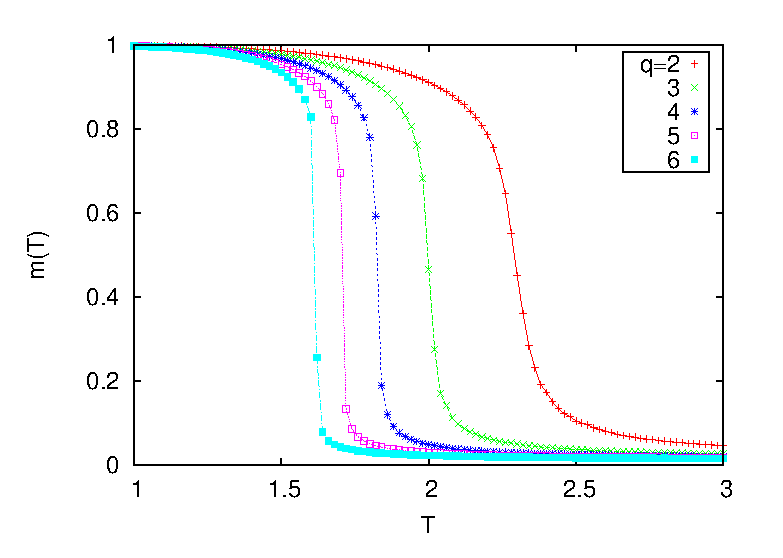
\includegraphics[width=14cm]{img/MagPotts.eps}
 \caption{Magnetização para o modelo de Potts, com $q=2, 3, 4, 5, 6$. Nota-se a presença de duas fases: uma desordenada, onde a magnetização é quase nula (fase paramagnética) e outra ordenada, onde a magnetização tem um valor próximo a $1$ (fase ferromagnética). Os resultados foram obtidos através de uma simulação usando o algoritmo do banho térmico, para uma rede bidimensional quadrada com dimensão linear $L=60$.}
\label{fig.MagPotts}
\end{figure}


\section{Domínios geométricos e \textit{hulls}}

Dois conceitos utilizados no estudo da morfologia de modelos de spins são os de domínios geométricos e \textit{hulls}, exemplificados na figura~\ref{fig.DomainsHulls}. Um domínio geométrico é definido como um agrupamento de spins com a mesma orientação, tal que quaisquer dois spins pertencentes ao mesmo podem ser conectados por um caminho composto de outros spins com a mesma orientação, e que pode ser percorrido com passos entre primeiros vizinhos. A área do domínio corresponde à superfície desse agrupamento, que no caso de spins discretos corresponde ao número de spins contidos no agrupamento. Domínios geométricos podem conter e estar contidos em outros domínios geométricos. Um \textit{hull} é definido como o contorno externo de um domínio geométrico, e sua área corresponde à área desse domínio geométrico, mais as áreas de todos os outros domínios geométricos por ele englobados.

A justificativa para a introdução do conceito de \textit{hull}, que pode parecer menos natural que o conceito de domínio geométrico, reside no fato que a determinação das áreas dos \textit{hulls} é um problema mais facilmente tratável por métodos analíticos, por essas áreas dependerem de uma única interface, facilitando assim a obtenção de expressões exatas.

Embora outros tipos de domínios sejam também utilizados em estudos relacionados a modelos de spins, como domínios de Fortuin-Kasteleyn~\cite{FortuinKasteleyn}, o presente trabalho se limita a estudar propriedades associadas aos domínios geométricos (podendo aqui ser chamados simplesmente de domínios).

\begin{figure}
 \centering
 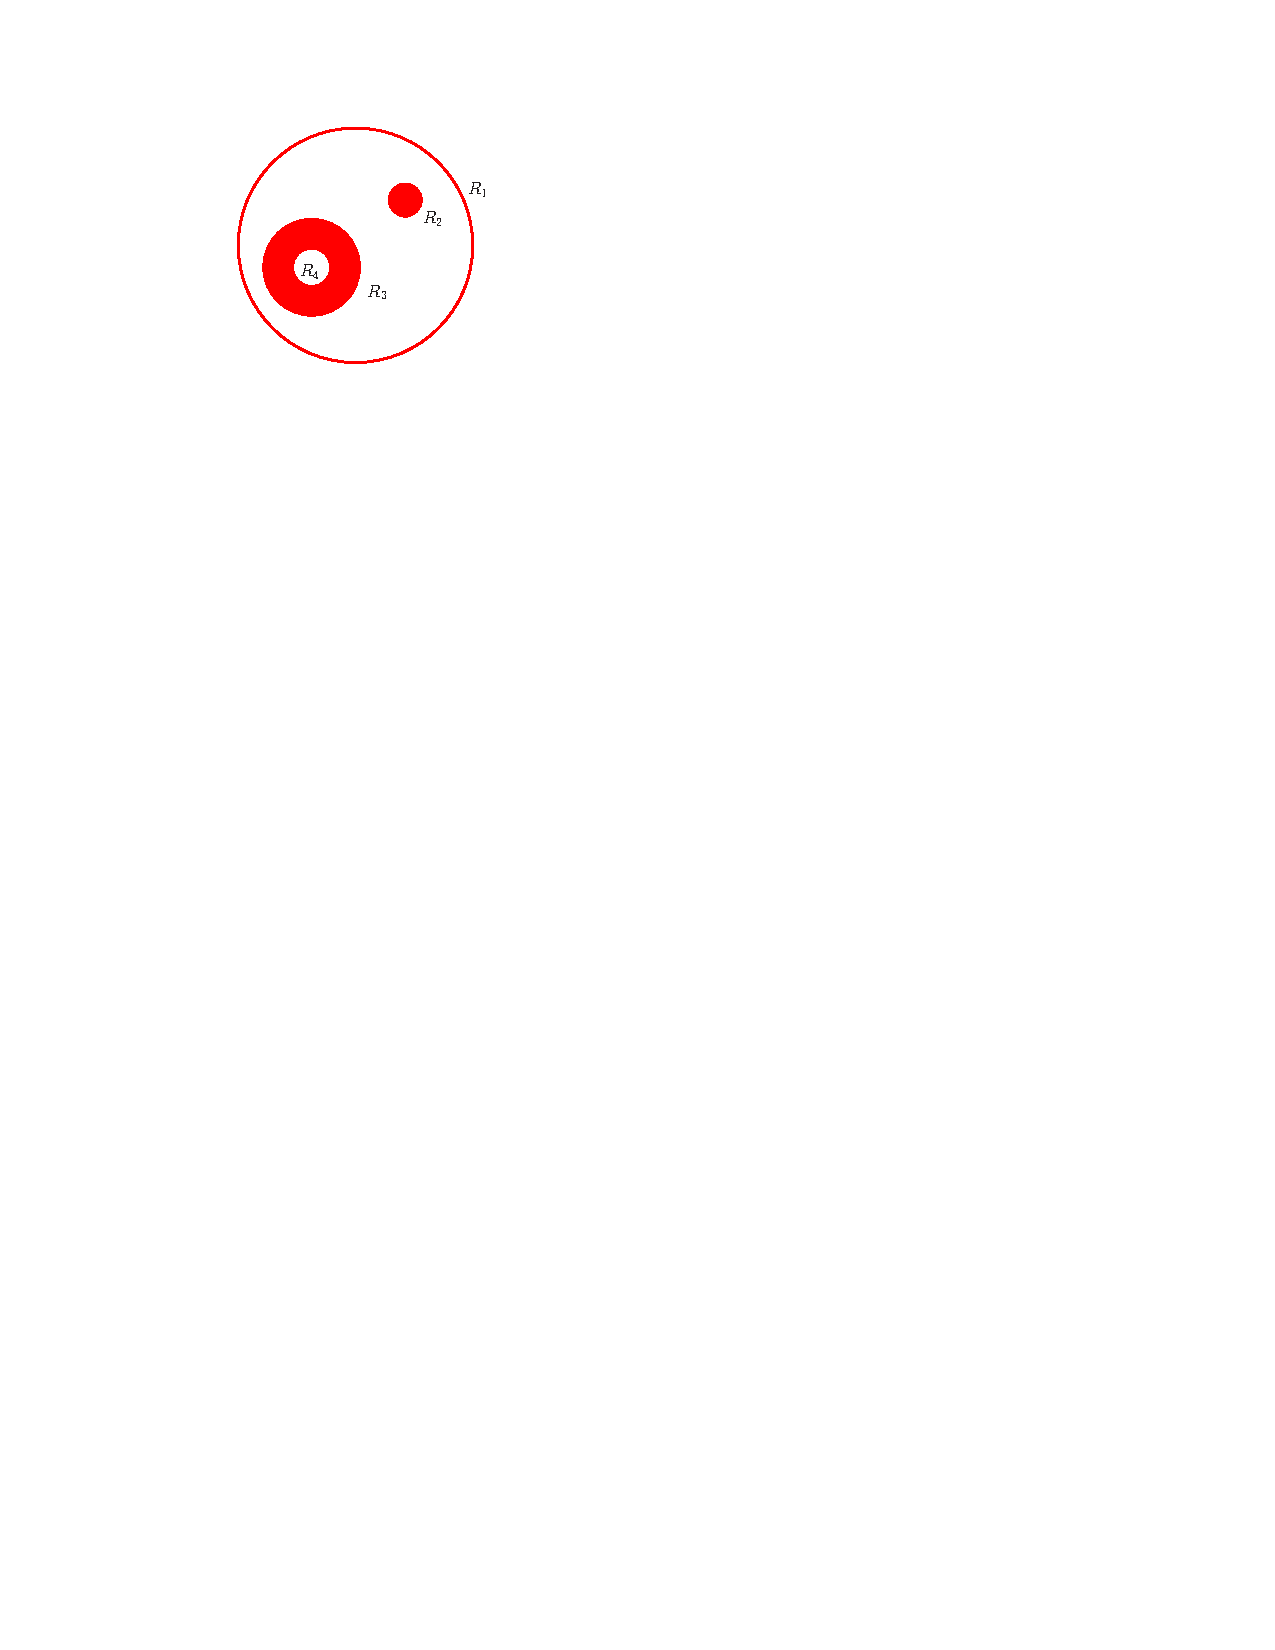
\includegraphics[width=6cm]{img/DomainsHulls.pdf}
 \caption{Exemplo de configuração com quatro \textit{hulls} e quatro domínios geométricos circulares. O \textit{hull} mais externo, de raio $R_1$, contém dois \textit{hulls} de primeira geração, de raios $R_2$ e $R_3$, e um \textit{hull} de segunda geração, de raio $R_4$. O \textit{hull} de raio $R_1$ engloba uma área de $\pi R_1^2$, enquanto que o domínio geométrico de raio $R_1$ tem uma área de $\pi(R_1^2-R_2^2-R_3^2)$~\cite{PREJeferson}.}
\label{fig.DomainsHulls}
\end{figure}


\section{Escalamento dinâmico}

Observa-se em diversos sistemas que apresentam uma dinâmica de crescimento de domínios, ao evoluírem fora do equilíbrio, tanto experimentalmente como em simulações numéricas, que as estruturas formadas pelos domínios são estatisticamente similares em diferentes tempos, a menos de um fator de escala global. Essa observação levou à formulação da hipótese fenomenológica do escalamento dinâmico, que afirma que existe no sistema um único comprimento característico $R(t)$, que cresce com o tempo, de forma que o padrão das estruturas é estatisticamente independente do tempo quando todos os comprimentos são especificados em unidades de $R(t)$~\cite{ReviewBray}. Lifshitz e Slyozov~\cite{Lifshitz1961,Lifshitz1962} determinaram que em sistemas nos quais o parâmetro de ordem não é conservado, o que inclui os modelos de Ising e de Potts (para qualquer valor de $q$) conforme aqui apresentados, o comprimento característico $R(t)$ é bem descrito por:
\begin{equation}
 R(t) \sim t^{1/2}. 
\end{equation}


\section{Dinâmica de crescimento}

Observa-se no modelo de Ising, após um \textit{quench} através da temperatura crítica, uma dinâmica de crescimento de domínios, conforme se pode observar na figura \ref{fig.IsingSnap}.

\begin{figure}[h!]
 \setlength\fboxsep{0pt}
 \setlength\fboxrule{0.5pt}
 \centering
 \fbox{
\includegraphics[width=35mm]{img/Ising_scr1.png}}
 \fbox{
\includegraphics[width=35mm]{img/Ising_scr2.png}}
 \fbox{
\includegraphics[width=35mm]{img/Ising_scr3.png}}
 \fbox{
\includegraphics[width=35mm]{img/Ising_scr4.png}} \\
 (a) \hspace{30mm} (b) \hspace{30mm} (c) \hspace{30mm} (d) \vspace{3mm} \\
 \caption{Sequência mostrando a evolução de uma simulação de Monte Carlo do modelo de Ising, após um \textit{quench} da temperatura infinita para a temperatura zero. Os respectivos tempos são $t=2,8,32,256$ passos de Monte Carlo (MCs). Pontos pretos e brancos representam spins com valores $-1$ e $+1$. Para $t \rightarrow \infty$ o sistema atinge ou um estado ordenado, ou um estado formado por listras de spins com a mesma orientação~\cite{BlanchardPicco}.}
 \label{fig.IsingSnap}
\end{figure}

Em 1979, Allen e Cahn~\cite{AllenCahn} verificaram que a velocidade de um elemento de área de uma interface entre dois domínios, para sistemas com parâmetro de ordem não conservado, está relacionada à curvatura local dessa interface, obtendo a relação, válida para qualquer dimensão:
\begin{equation}
 \label{eq.AllenCahn}
 v=-\frac{\lambda}{2\pi} \kappa,
\end{equation}
onde $\lambda$ é um parâmetro dependente da temperatura, com dimensões de constante de difusão, $\kappa$ a curvatura local, e $v$ a velocidade do elemento de área da interface, normal a cada ponto da mesma, com sentido na direção que determina a redução da curvatura.

Podemos expressar a variação da área englobada por um \textit{hull} através de uma integral de caminho, sobre o \textit{hull}, da velocidade de um elemento diferencial do mesmo:
\begin{equation}
 \label{eq.DaDtq2}
 \frac{dA_h}{dt} = \oint v dl = -\frac{\lambda_h}{2\pi} \oint \kappa dl = -\lambda_h,
\end{equation}
onde\footnote{Utilizamos aqui $\lambda_h$ para denotar o parâmetro associado com a variação de áreas englobadas por \textit{hulls}, enquanto que para o caso de domínios geométricos, o parâmetro será denotado por $\lambda_d$.} a última igualdade é obtida a partir do teorema de Gauss-Bonnet~\cite{PRLJeferson}. Integrando a Eq.~(\ref{eq.DaDtq2}) no tempo, chega-se a:
\begin{equation}
 \label{eq.Area}
 A_h(t) = A_h(0) - \lambda_h t.
\end{equation}
Ou seja, independentemente de suas áreas, todos os \textit{hulls} diminuem com a mesma taxa. Definindo $n_h(A,t)$ como a distribuição das áreas dos \textit{hulls}, tal que $n_h(A, t)dA$ é o número de \textit{hulls} com áreas entre $A$ e $A+dA$ no tempo $t$, usando a Eq.~(\ref{eq.Area}), temos:
\begin{equation}
 \label{eq.DistHulls}
 n_h(A,t) = n_h(A+\lambda_h t,0).
\end{equation}

Observa-se que, conhecida a distribuição inicial das áreas dos \textit{hulls}, pode-se determinar a distribuição em qualquer tempo subsequente, e que a distribuição mantém a sua forma durante a evolução temporal, apenas se deslocando na direção de áreas menores.


\section{Distribuições de áreas de \textit{hulls} para $q=2$}

A forma da distribuição das áreas dos \textit{hulls} para o modelo com dois estados (Ising, ou, equivalentemente, Potts com $q=2$), para a condição de equilíbrio na temperatura crítica, foi determinada por Cardy e Ziff em 2003~\cite{Cardy2003}. A expressão obtida para esse caso equivale a:
\begin{equation}
 \label{eq.hq2t0Tc}
 n_h(A,0) \sim \frac{c_h}{A^2}, \qquad T_0 = T_c,
\end{equation}
onde $c_h = 1/(8\pi\sqrt{3})$ é uma constante universal. A expressão é válida para $A_0 \ll A \ll L^2$, sendo $A_0$ uma área microscópica, da ordem de grandeza da área ocupada por uma partícula, e $L^2$ o tamanho do sistema.

Cardy e Ziff determinaram ainda a forma da distribuição das áreas dos \textit{hulls} para um modelo de percolação aleatória na densidade crítica. Um modelo de percolação aleatória pode ser definido sobre uma rede com determinada geometria, onde cada sítio pode estar ocupado por uma partícula ou vazio, com uma distribuição aleatória das partículas, sendo que sítios ocupados adjacentes (primeiros vizinhos) são considerados como pertencentes a um mesmo agrupamento, \textit{cluster} ou domínio, sendo os \textit{hulls} definidos da mesma forma que para os modelos de spins. Para uma densidade de ocupação de sítios $\rho$ maior que determinada densidade crítica $\rho_c$, surge no sistema um domínio de dimensões macroscópicas (ou percolante), que ocupa uma fração finita do tamanho total do sistema (sendo infinito, para um sistema infinito)~\cite{Stauffer}. A expressão encontrada para a distribuição das áreas dos \textit{hulls} para esse caso foi a mesma encontrada para o modelo de dois estados para a condição de equilíbrio na temperatura crítica, ou seja:
\begin{equation}
 \label{eq.nrandperc}
 n_p(A) \sim \frac{c_h}{A^2}, \qquad \rho = \rho_c.
\end{equation}

Embora a distribuição das áreas dos \textit{hulls} para o modelo com dois estados, para a temperatura infinita, não seja conhecida exatamente, Arenzon \textit{et al}~\cite{PRLJeferson} mostraram, através de simulações, que o estado do modelo nessas condições se aproxima rapidamente do estado do modelo de percolação aleatória na densidade crítica. Esse comportamento pode ser explicado por termos, quando $T \rightarrow \infty$, uma igual probabilidade de encontrar os spins em cada um dos dois possíveis estados. Podemos assim estabelecer uma correspondência entre os dois estados possíveis do spin e os estados possíveis de um sítio no modelo de percolação aleatória (ocupado ou vazio), e dizer que temos um caso equivalente ao do modelo de percolação aleatória com uma densidade de ocupação $\rho = 1/2$, que se aproxima do valor da densidade crítica $\rho_c$. Assim, temos:
\begin{equation}
 \label{eq.hq2t0Tinf}
 n_h(A,0) = 2 n_p(A) \sim \frac{2c_h}{A^2}, \qquad T_0 \rightarrow \infty,
\end{equation}
onde o fator 2 se justifica pela existência de dois tipos de domínios, correspondentes aos dois estados do modelo, enquanto que o resultado obtido para o modelo de percolação aleatória considera apenas domínios de sítios ocupados (e não domínios de sítios vazios)~\cite{PRLJeferson}.

Considerando as Eq.~(\ref{eq.hq2t0Tc}) e (\ref{eq.hq2t0Tinf}) como condições iniciais da Eq.~(\ref{eq.DistHulls}), chega-se a:
\begin{equation}
 \label{eq.hq2tTinf}
 n_h(A,t) = \frac{2c_h}{\left(A + \lambda_h t \right)^2}, \qquad T_0 \rightarrow \infty,
\end{equation}
\begin{equation}
 \label{eq.hq2tTc}
 n_h(A,t) = \frac{c_h}{\left(A + \lambda_h t\right)^2}, \qquad T_0 = T_c.
\end{equation}

As distribuições dadas pelas Eq.~(\ref{eq.hq2tTinf}) e (\ref{eq.hq2tTc}) correspondem a sistemas com áreas características proporcionais a $t$, ou comprimentos característicos proporcionais a $t^{1/2}$, validando o resultado previsto pela hipótese de escalamento dinâmico.


\section{Distribuições de áreas de domínios geométricos para $q=2$}
\label{sec.DistAreasDomGeo}

Arenzon \textit{et al}~\cite{PRLJeferson,PREJeferson} mostraram que as formas das distribuições de áreas de domínios geométricos são similares às obtidas para as áreas dos \textit{hulls}, sendo descritas pelas expressões:
\begin{equation}
 \label{eq.dq2tTinf}
 n_d(A,t) = \frac{2c_d}{\left(A + \lambda_d t \right)^{\tau^\prime}}, \qquad T_0 \rightarrow \infty,
\end{equation}
\begin{equation}
 \label{eq.dq2tTc}
 n_d(A,t) = \frac{c_d}{\left(A + \lambda_d t\right)^\tau}, \qquad T_0 = T_c,
\end{equation}
onde $\tau^\prime = 187/91 \approx 2.055$, $\tau = 379/187 \approx 2.027$, e $c_d \approx c_h$. Na figura \ref{fig.areas_q2_L256} pode-se observar uma comparação entre resultados descritos pelas Eq.~(\ref{eq.dq2tTinf}) e (\ref{eq.dq2tTc}), e obtidos através de simulações numéricas baseadas no método de Monte Carlo.

\begin{figure}[h!]
 \centering
 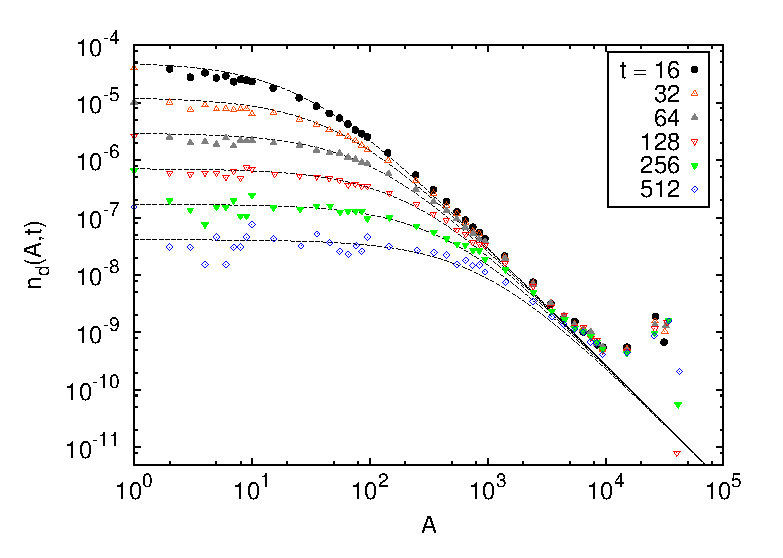
\includegraphics[width=14cm]{fig/areas_q2_L256_Tinf_T0.eps} \\
 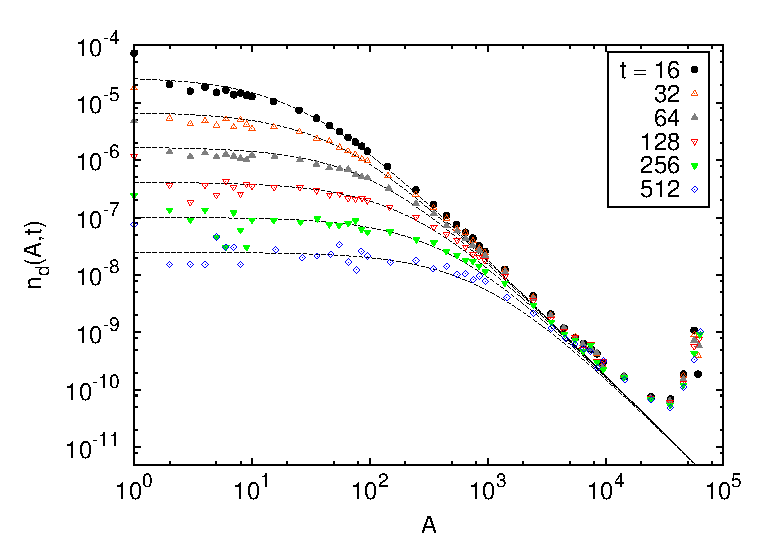
\includegraphics[width=14cm]{fig/areas_q2_L256_Tc_T0.eps}
 \caption{Distribuições das áreas dos domínios geométricos para $q=2$, em diferentes tempos, após um \textit{quench} de um estado de equilíbrio na temperatura inicial para $T_f=0$, para duas condições de temperatura inicial: no gráfico superior para $T_0 \rightarrow \infty$ e no inferior para $T_0 = T_c$. As linhas tracejadas correspondem a valores dados pelas Eq.~(\ref{eq.dq2tTinf}) e (\ref{eq.dq2tTc}), com $\lambda_d = 2.15$, enquanto os pontos resultam de simulações utilizando o método de Monte Carlo para uma rede quadrada com dimensão linear $L=256$, com uma média sobre 4000 amostras para cada caso. Os pontos que desviam das curvas, para áreas grandes, podem ser explicados pela existência de domínios percolantes, limitados pelas dimensões finitas da rede e computados com áreas menores do que teriam na ausência da limitação. Como o sistema é pequeno, vemos somente o início do comportamento do tipo lei de potência, esperado para grandes áreas.}
 \label{fig.areas_q2_L256}
\end{figure}


\section{Dinâmica para $q>2$}

Observa-se em sistemas com degenerescência múltipla no estado fundamental uma dinâmica de crescimento de domínios, após um \textit{quench} sobre a temperatura crítica, análoga à observada para sistemas com dupla degenerescência, conforme se pode observar na figura \ref{fig.PottsSnap}. Permanece válida a Eq.~(\ref{eq.AllenCahn}), sendo o parâmetro $\lambda$ dependente de $q$ e da temperatura.

\begin{figure}[h!]
 \setlength\fboxsep{0pt}
 \setlength\fboxrule{0.5pt}
 \centering
 \fbox{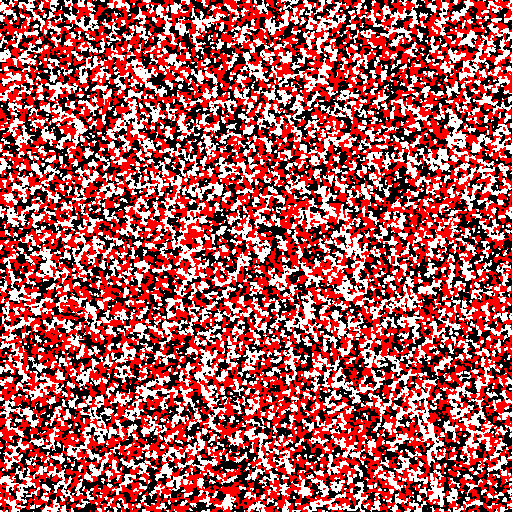
\includegraphics[width=35mm]{img/Potts_scr1.png}}
 \fbox{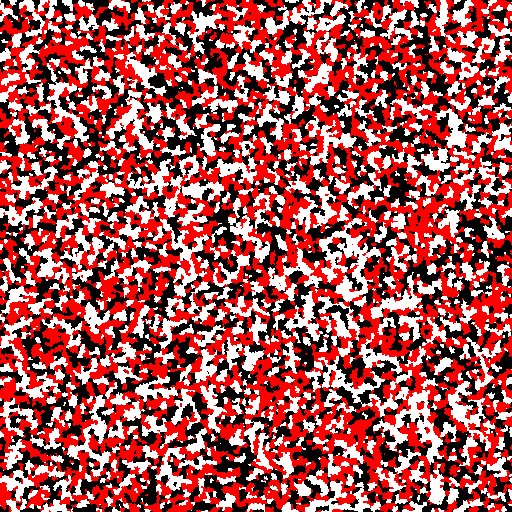
\includegraphics[width=35mm]{img/Potts_scr2.png}}
 \fbox{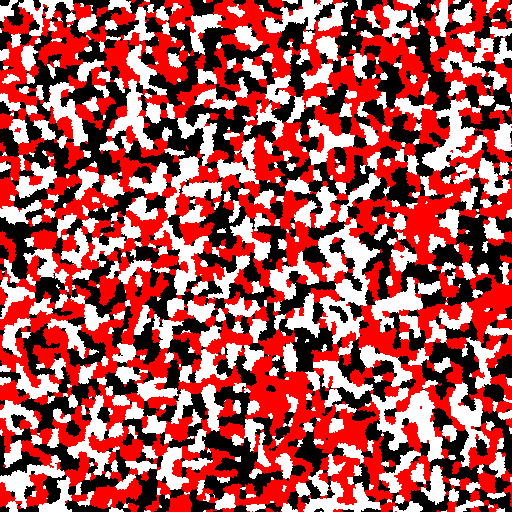
\includegraphics[width=35mm]{img/Potts_scr3.png}}
 \fbox{
\includegraphics[width=35mm]{img/Potts_scr4.png}} \\
 (a) \hspace{30mm} (b) \hspace{30mm} (c) \hspace{30mm} (d) \vspace{3mm} \\
 \caption{Sequência mostrando a evolução de uma simulação de Monte Carlo do modelo de Potts com $q=3$, após um \textit{quench} da temperatura infinita para a temperatura zero. Os respectivos tempos são $t=2,8,32,256$ passos de Monte Carlo (MCs). Pontos pretos, brancos e vermelhos representam os diferentes estados possíveis para cada spin.}
 \label{fig.PottsSnap}
\end{figure}

Pode-se expressar a variação da área englobada por um \textit{hull} através de uma integral de caminho, sobre o \textit{hull}, da velocidade de um elemento diferencial do mesmo, de forma análoga ao que foi descrito para o caso com dupla degenerescência:
\begin{equation}
 \label{eq.DaDtq3}
 \frac{dA_h}{dt} = \oint v dl = -\frac{\lambda_h}{2\pi} \oint \kappa dl = -\lambda_h \left(1-\frac{1}{2\pi}\sum_i\alpha_i \right),
\end{equation}
onde a última igualdade é obtida a partir da forma geral do teorema de Gauss-Bonnet, e os $\alpha_i$ são os menores ângulos entre as retas tangentes às superfícies nos $n$ vértices ou junções triplas~\cite{LoureiroPRE}, conforme pode ser visto na figura~\ref{fig.GaussBonnet}. No caso $q=2$ não existem vértices, e a Eq.~(\ref{eq.DaDtq3}) se reduz à Eq.~(\ref{eq.DaDtq2}).

\begin{figure}
 \centering
 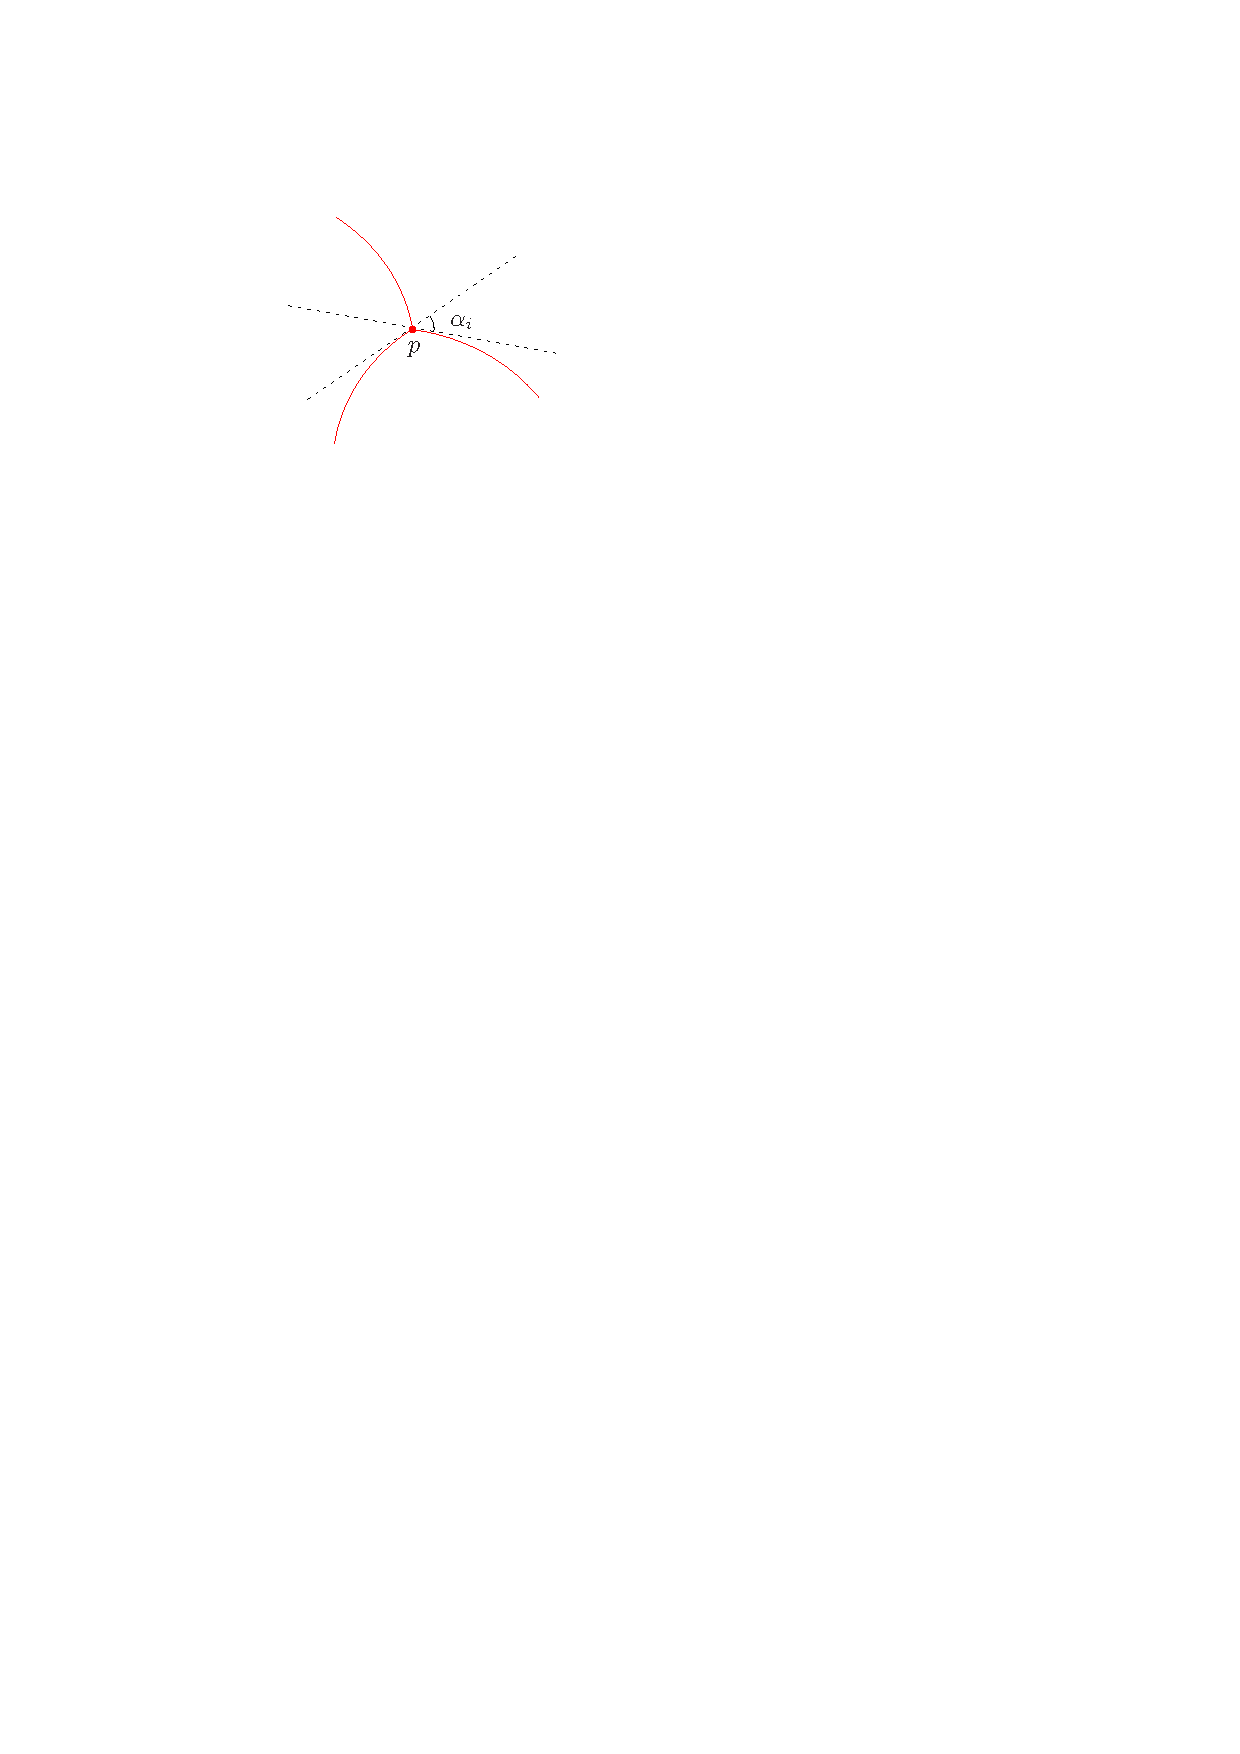
\includegraphics[width=70mm]{img/gauss_bonnet1.pdf}
 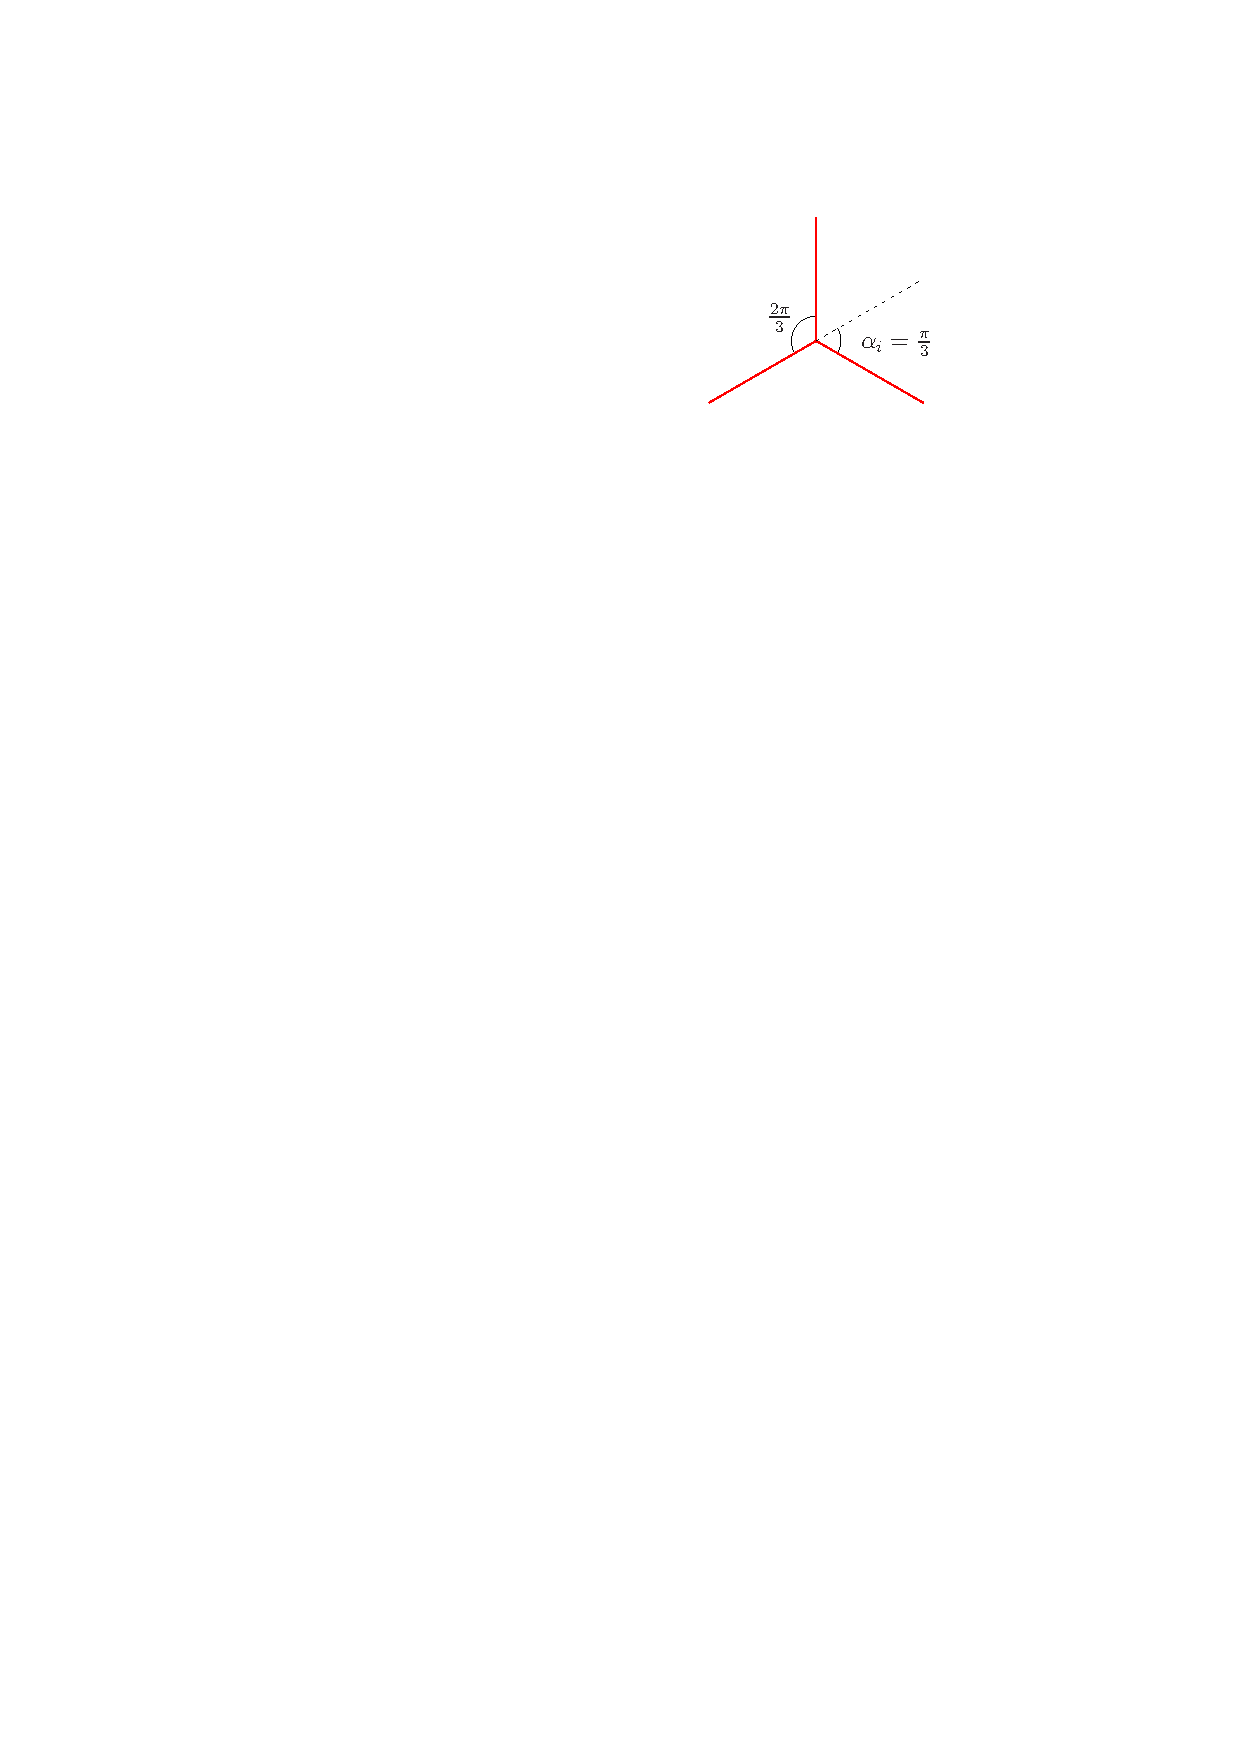
\includegraphics[width=70mm]{img/gauss_bonnet2.pdf} \\
 (a) \hspace{60mm} (b)
 \caption{Representação de vértices ou junções triplas. Em (a) temos o ângulo $\alpha_i$, que é o menor ângulo entre retas tangentes às interfaces entre domínios, no ponto $p$. Em (b) temos uma configuração análoga, no limite em que todos os ângulos entre domínios, nos pontos de junções triplas, são iguais a $2\pi/3$ ($\alpha_i = \pi/3$)~\cite{TeseMP}.}
 \label{fig.GaussBonnet}
\end{figure}

Para alguns sistemas, como modelos de espumas, os ângulos entre domínios, nos pontos de junções triplas, são todos iguais a $2\pi/3$. Restringindo a análise a sistemas desse tipo, ou que possam assim ser aproximados, e considerando uma correspondência de um para um entre vértices e lados, a Eq.~(\ref{eq.DaDtq3}) se reduz à lei de von Neumann~\cite{Neumann1952,Mullins1956} para a área $A_n$ de um \textit{hull} de $n$ lados:
\begin{equation}
 \label{eq.vonNeumann}
 \frac{dA_n}{dt} = \frac{\lambda}{6} \left( n-6 \right).
\end{equation}

Observando-se a Eq.~(\ref{eq.vonNeumann}), percebe-se que a evolução da área de um \textit{hull} depende fundamentalmente do número $n$ de lados do mesmo: para $n<6$ a área decresce, para $n>6$ ela cresce, e para $n=6$ se mantém constante. Domínios com poucos vizinhos tendem a diminuir e desaparecer, ao contrário dos com muitos vizinhos. Além disso, o número de lados de um \textit{hull} pode variar durante a evolução do sistema, à medida que seus domínios vizinhos evoluem ou desaparecem. Dessa forma, diferentemente do caso $q=2$, para $q>2$, em princípio não é possível obter uma expressão exata que determine a área de um \textit{hull} em um tempo $t$ qualquer, sendo conhecida sua área inicial~\cite{LoureiroPRE,LoureiroPRE2012}. No entanto, verifica-se que em determinados casos, como o do modelo com $q=3$, após um \textit{quench} a partir de um estado de equilíbrio em $T_0=T_c$, o sistema apresenta distribuições de \textit{hulls} e domínios geométricos com o mesmo comportamento observado para o caso $q=2$.

Na figura \ref{fig.AreasCol}, pode-se observar distribuições de áreas de domínios geométricos para $q=2$ e $q=3$, com $T_0 \rightarrow \infty$ e $T_0=T_c$, colapsadas para diversos tempos. O colapso obtido com o fator de escala $A \Rightarrow A/t$ era esperado, de acordo com a hipótese de escalamento dinâmico. Pode-se verificar que no caso $q=3$ com $T_0=T_c$, o colapso dos pontos se apresenta na forma esperada para uma dinâmica descrita pela Eq.~(\ref{eq.dq2tTc}), embora em princípio a mesma se aplique apenas ao caso $q=2$. A explicação definitiva para tal comportamento é ainda uma questão em aberto~\cite{LoureiroPRE}. Para o caso $q=3$ com $T_0 \rightarrow \infty$, a distribuição não apresenta cauda longa, não tendo uma forma compatível com a Eq.~(\ref{eq.dq2tTc}). Os dados utilizados na construção da figura \ref{fig.AreasCol} não incluem pontos associados com domínios percolantes, o que faz com que a distribuição não apresente picos para grandes tamanhos de domínios, como acontece na figura \ref{fig.areas_q2_L256}, mas apresente um desvio para baixo.

A temperatura final do \textit{quench} foi definida como $T_f=T_c/2$, em todos os casos. Assim evita-se o efeito de \textit{pinning}, que ocorre para $q > 2$, para temperaturas muito baixas, e que consiste no aparecimento de pontos ou regiões estáveis que interrompem a dinâmica~\cite{DerridaOliveiraStauffer}. Ao mesmo tempo, é suficientemente baixa para que permaneçam aplicáveis expressões que foram derivadas sem levar em consideração explicitamente a presença de flutuações térmicas.

\begin{figure}
 \centering
 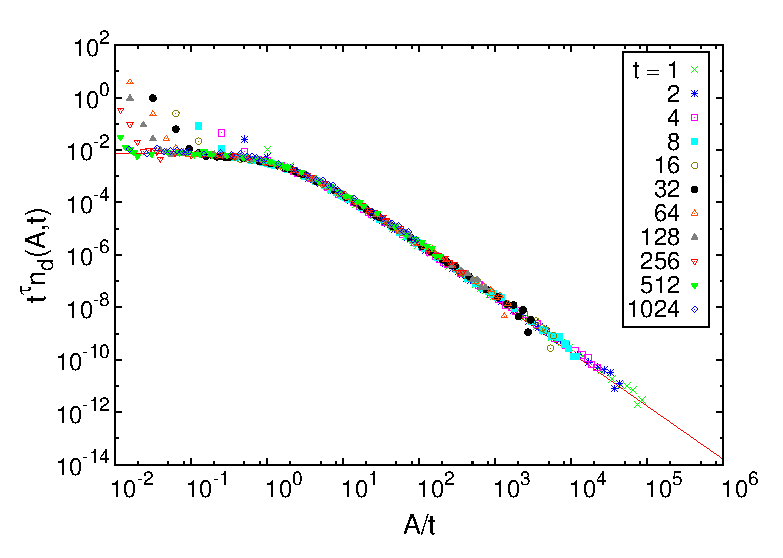
\includegraphics[width=7.65cm]{fig/areasnp_col_q2_L512_Tc_Tc2.eps}
 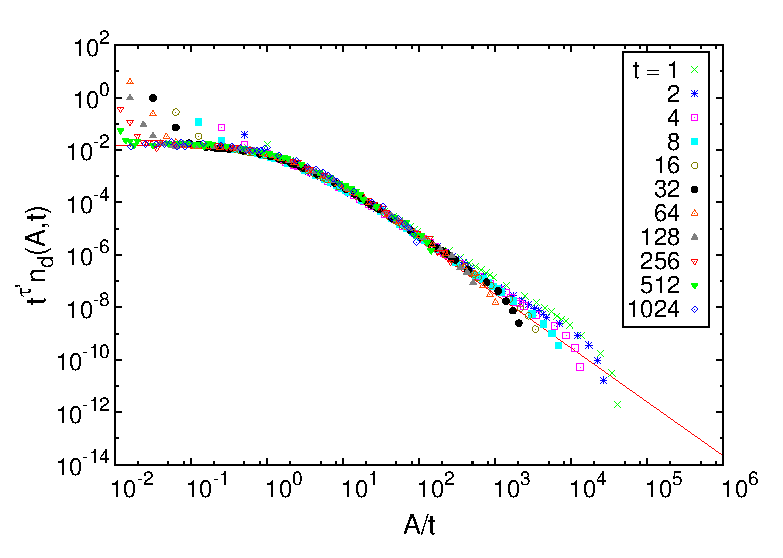
\includegraphics[width=7.65cm]{fig/areasnp_col_q2_L512_Tinf_Tc2.eps} \\
\hspace{8mm} (a) \hspace{70mm} (b)  \\
 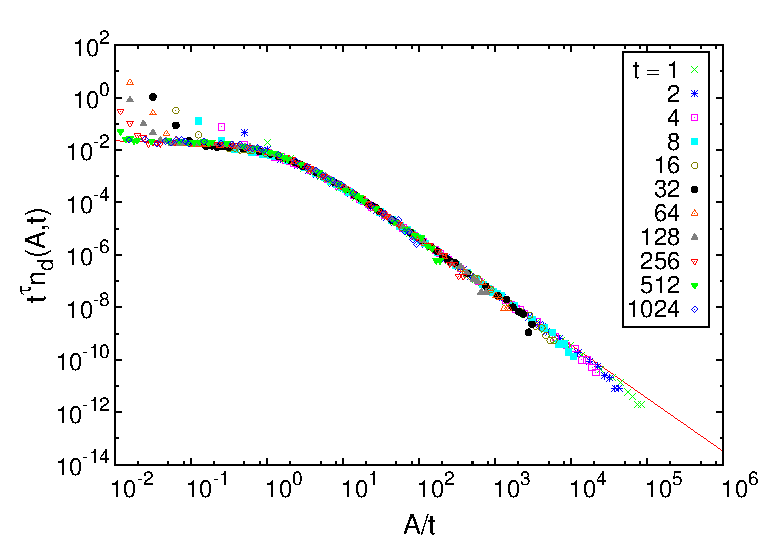
\includegraphics[width=7.65cm]{fig/areasnp_col_q3_L512_Tc_Tc2.eps}
 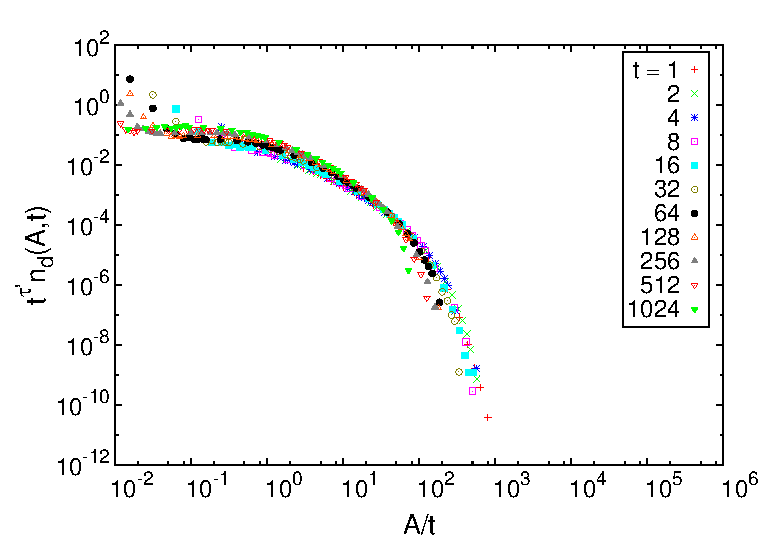
\includegraphics[width=7.65cm]{fig/areasnp_col_q3_L512_Tinf_Tc2.eps} \\
\hspace{8mm} (c) \hspace{70mm} (d)
 \caption{Distribuições das áreas dos domínios geométricos, colapsadas para diversos tempos. Em (a) e (b), para $q=2$ e em (c) e (d) para $q=3$. Em (a) e (c) o sistema sofreu um \textit{quench} a partir de um estado de equilíbrio em $T_0=T_c$ para $T_f=T_c/2$, enquanto que em (b) e (d) o \textit{quench} ocorreu de um estado de equilíbrio em $T_0 \rightarrow \infty$ para $T_f=T_c/2$. Os pontos resultam de simulações utilizando o método de Monte Carlo para uma rede quadrada com dimensão linear $L=512$, com uma média sobre 1000 amostras para cada caso. Os domínios percolantes não foram incluídos nas distribuições. As linhas sólidas correspondem a valores dados pelas Eq.~(\ref{eq.dq2tTinf}) e (\ref{eq.dq2tTc}), com mudanças nos parâmetros para o caso $q=3$.}
 \label{fig.AreasCol}
\end{figure}


\chapter{Heterogeneidade em estados de equilíbrio}
\label{cap.Heterogeneidade}

\section{Introdução}

O conceito de heterogeneidade de tamanhos de domínios foi inicialmente introduzido no contexto de um modelo de grafo aleatório~\cite{LeeKimPark}, construído através da introdução de uma modificação no modelo de Erdős-Rényi~\cite{Achlioptas}. O modelo de Erdős-Rényi descreve um particular processo de construção de um grafo aleatório: inicia-se com $N$ vértices isolados e adicionam-se ligações entre os mesmos, uma a cada passo, através da escolha aleatória de dois vértices. Com a sucessiva adição de novas ligações, surgem domínios de vértices conectados. A heterogeneidade de tamanhos de domínios é definida como o número de tamanhos distintos de domínios existentes em determinada configuração de um sistema, sendo o tamanho de um domínio dado pelo número de vértices contidos no mesmo.

Definindo como um parâmetro de controle do sistema uma densidade de ligações $t \equiv K/N$, sendo $K$ o número de ligações, verifica-se que para um determinado valor $t_c$, o modelo apresenta uma transição de fase, denominada transição de percolação, caracterizada pelo aparecimento de um domínio de dimensões macroscópicas (componente gigante), definido como um domínio que escala com $N$. Definindo-se um parâmetro de ordem $g(t) \equiv G(t)/N$, onde $G(t)$ é o tamanho do maior domínio, verifica-se que no limite $N \rightarrow \infty$, para $t < t_c$ temos $g(t)=0$, enquanto que para $t > t_c$, $g(t)$ tem um valor finito, evidenciando a presença de duas fases distintas, sendo a transição entre uma fase e outra contínua.

O modelo descrito na Ref.~\cite{Achlioptas} define um método alternativo para a construção do grafo: partindo-se de $N$ vértices isolados, a cada passo escolhe-se aleatoriamente dois pares de vértices, escolhendo-se então, entre os dois pares, para a construção de uma nova ligação, aquele que minimiza o produto dos tamanhos dos domínios a serem conectados. O modelo baseado nessa \textit{regra do produto} atraiu considerável interesse, por exibir uma transição de fase aparentemente descontínua, diferentemente do que é encontrado no modelo de Erdős-Rényi e outros modelos de percolação, tendo sido denominado este comportamento de percolação explosiva. O caráter contínuo ou descontínuo da transição foi elucidado no trabalho de Lee \textit{et al}~\cite{LeeKimPark}, onde foi demonstrado que, assim como as transições observadas nos modelos mais tradicionais de percolação, a transição na percolação explosiva era também contínua. A figura \ref{fig.ErdosProduct} ilustra o processo de construção de um grafo de acordo com os modelos de Erdős-Rényi e da regra do produto.

\begin{figure}
 \centering
 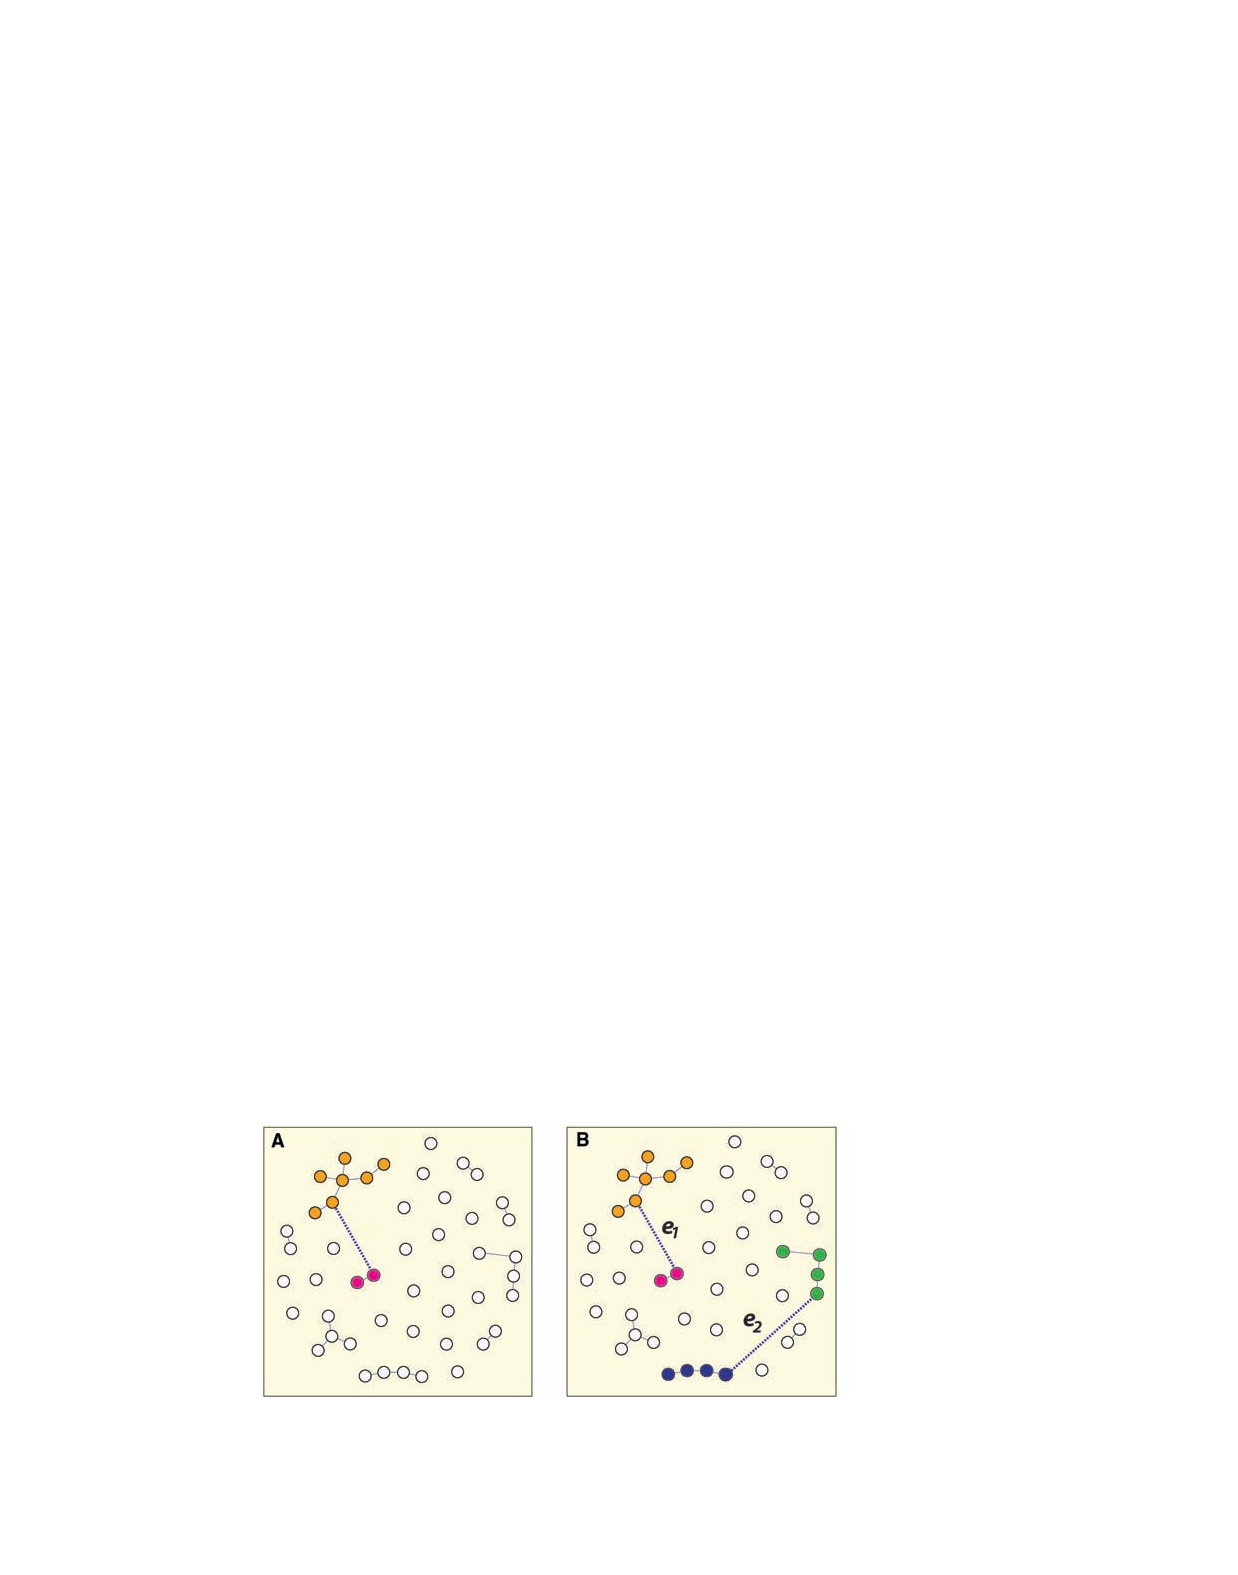
\includegraphics[width=14cm]{img/ErdosProduct.pdf}
 \caption{Processo de construção do grafo. (A) no modelo de Erdős-Rényi, a cada passo, dois vértices são selecionados aleatoriamente e conectados por uma nova ligação. (B) em modelos que incorporam um determinado grau de escolha, a cada passo, dois pares de vértices são selecionados aleatoriamente e um dos pares é escolhido de acordo com alguma regra, como a regra do produto, e então conectado por uma nova ligação, enquanto que o outro par é desconsiderado~\cite{Achlioptas}.}
\label{fig.ErdosProduct}
\end{figure}

O argumento descrito por Lee \textit{et al} utiliza dois pseudo-pontos de transição, $t_l$ e $t_u$, definidos respectivamente como limites inferior e superior para o real ponto de transição $t_c$, convergindo assintoticamente ao mesmo no limite $N \rightarrow \infty$. O ponto $t_l$ foi definido como o ponto em que se observa um máximo na heterogeneidade dos tamanhos de domínios de vértices conectados. No estado inicial do grafo, existe apenas um tamanho de domínio (domínios formados por vértices isolados). Com a adição de novas ligações, e consequente aumento do parâmetro de controle $t$, vão surgindo outros tamanhos de domínios no sistema, e a medida de heterogeneidade aumenta. Entretanto, a partir de determinado ponto, aparece um domínio de dimensões macroscópicas que começa a absorver domínios menores, levando a uma progressiva redução da heterogeneidade, até que, eventualmente, exista um único domínio contendo todos os vértices. Como a regra do produto torna desfavorável o aparecimento de domínios grandes, espera-se que a heterogeneidade aumente lentamente, mas constantemente, com o aumento de $t$, até um ponto imediatamente antes do ponto $t_c$, em que domínios de diferentes tamanhos são combinados em um grande domínio~\cite{LeeKimPark}. O ponto $t_u$ foi definido como o ponto imediatamente subsequente ao ponto em que o tamanho do segundo maior domínio tem seu valor máximo. Os autores utilizaram simulações numéricas para validar as hipóteses acerca do comportamento dos pontos $t_l$ e $t_u$. A figura \ref{fig.tltu} mostra a variação dos valores de $t_l$ e $t_u$ com o aumento de $N$.

\begin{figure}
 \centering
 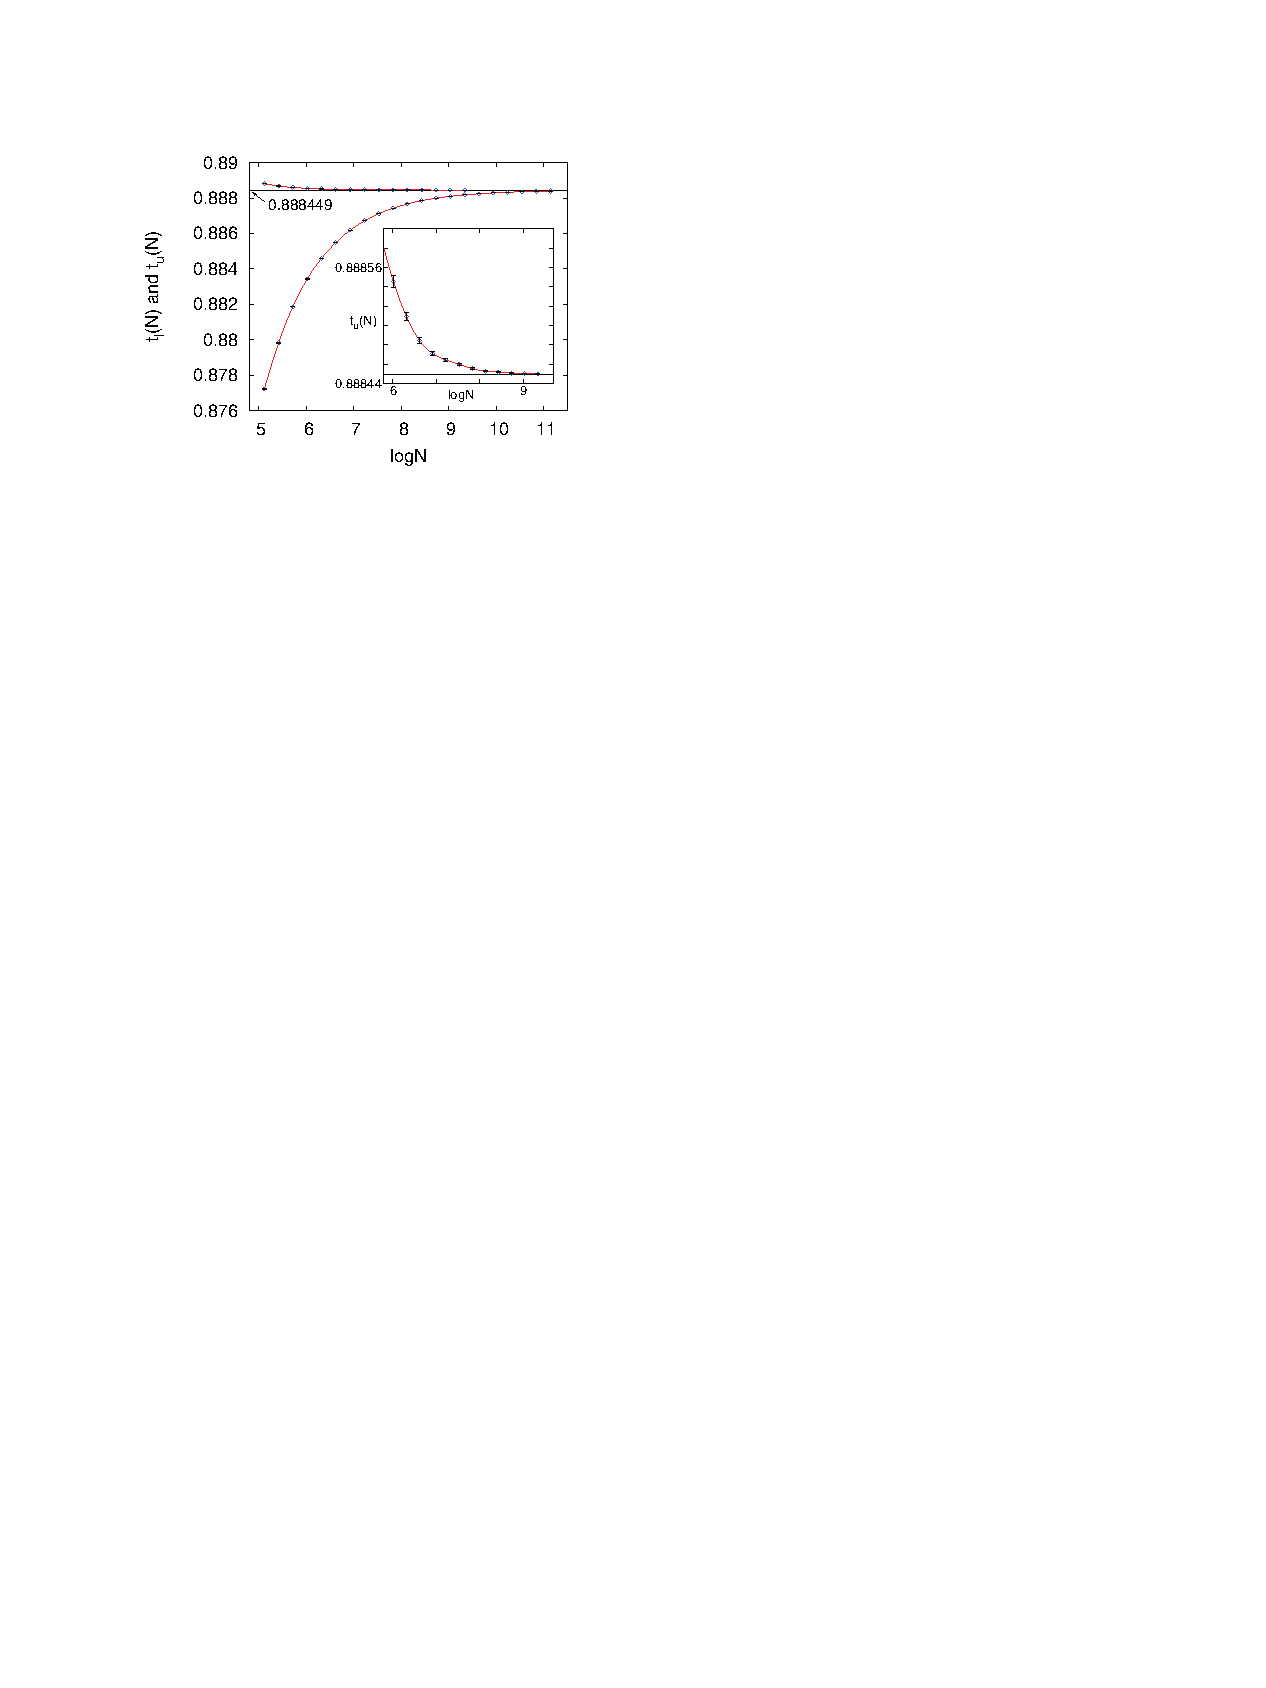
\includegraphics[width=14cm]{img/tltu.pdf}
 \caption{Variação de $t_l$ (ramo inferior) e $t_u$ (ramo superior) com o tamanho do sistema. No limite termodinâmico, $t_l$ e $t_u$ convergem para o valor de $t_c = 0.8884490(5)$~\cite{LeeKimPark}.}
\label{fig.tltu}
\end{figure}

A Ref.~\cite{LeeKimPark} utiliza a definição de $t_l$ e $t_u$ em um argumento que não será detalhado aqui, determinando um limite superior para o aumento de tamanho sofrido pelo maior domínio entre os pontos $t_l$ e $t_u$, verificando que esse aumento é sub-linear em $N$, o que implica a inexistência de um salto finito no valor do parâmetro de ordem na transição de fase, no limite $N \rightarrow \infty$, refutando assim a hipótese de uma transição descontínua na percolação explosiva. 

O sucesso do uso da heterogeneidade de tamanhos de domínios no modelo de percolação explosiva motivou o estudo detalhado das propriedades dessa medida, bem como a sua aplicação a outros modelos, como modelos de percolação de ligações e de sítios~\cite{NohLeePark}, definidos sobre uma rede, assim como os modelos de Ising~~\cite{JoYiBaekKim} e de Potts~\cite{LvYangDeng}.


\section{Heterogeneidade em modelos de percolação de rede}

Dois dos mais estudados modelos de percolação são o modelo de percolação de ligações e o modelo de percolação de sítios, definidos sobre uma rede com determinada geometria. No primeiro, ligações são estabelecidas entre primeiros-vizinhos na rede com uma probabilidade $p$. As ligações definem domínios de sítios conectados. Já no modelo de percolação de sítios, os sítios da rede estão ocupados com uma probabilidade $p$, ou vazios com probabilidade $1-p$, sendo que sítios ocupados adjacentes (primeiros vizinhos) são considerados como pertencentes a um mesmo domínio. Em ambos os modelos, a partir de determinado valor crítico $p_c$ da probabilidade $p$, também chamado de limiar de percolação, aparece um domínio macroscópico, definido da mesma forma que para o modelo de Erdős-Rényi. Define-se o parâmetro de ordem $m$ como a fração dos sítios pertencentes ao domínio macroscópico.

Noh \textit{et al}~\cite{NohLeePark} estudaram a heterogeneidade de tamanhos de domínios nos modelos de percolação de sítios e de ligações, utilizando escalamento de tamanhos finitos (\textit{finite size scaling} - FSS), verificando que a mesma satisfaz a equação:
\begin{equation}
 \label{eq.HetPerc}
 H(\epsilon,L) = L^{d/\tau} f(|\epsilon| L^{1/\nu_H}),
\end{equation} 
onde $\epsilon \equiv p-p_c$, $L$ é o tamanho linear da rede, $d$ é o número de dimensões, $\tau$ é o chamado expoente de Fisher, que caracteriza a distribuição de tamanhos de domínios, $f$ é a função de escala associada à heterogeneidade, e $\nu_H$ é um novo expoente crítico. Para justificar essa lei de escala, Noh \textit{et al}~\cite{NohLeePark} e Jo \textit{et al}~\cite{JoYiBaekKim} apresentam o seguinte argumento. Embora a distribuição de tamanhos de domínios não seja em geral conhecida exatamente (uma exceção é quando $p=p_c$), a sua forma segue
\begin{equation}
n(A) \sim A^{-\tau} \exp(-A/A_c),
\end{equation}
onde\footnote{Cabe notar que o $\tau$ aqui utilizado corresponde ao $\tau^\prime$ definido na seção~\ref{sec.DistAreasDomGeo}.} $\tau=187/91$ e $A_c$ é o tamanho característico dos domínios. Devido ao termo exponencial, $A_c$ funciona como um parâmetro de corte (\textit{cutoff}) para a distribuição: somente os domínios com $A<A_c$ aparecem em número significativo e a distribuição, até esse ponto, segue a lei de potência $A^{-\tau}$. À medida que o sistema se aproxima do limiar de percolação, $A_c$ diverge e ficamos somente com a lei de potência. Isto define um expoente crítico $\sigma$, $A_c \sim |\epsilon|^{-1/\sigma}$. Portanto, se o sistema estiver longe do limiar crítico, a heterogeneidade coincidirá com $A_c$,
$$
H \sim A_c \sim |\epsilon|^{-1/\sigma},
$$ 
pois domínios com $A>A_c$ serão raros\footnote{$n(A)$, qualquer que seja, é proporcional ao número de domínios com tamanho $A$, portanto $\int_0^{A_c}n(A)dA$ será proporcional ao número total de domínios. Para contar apenas uma vez o tamanho $A$, devemos dividir o integrando por $n(A)$. Então temos: $H \sim \int_0^{A_c}\frac{n(A)}{n(A)}dA = A_c$.}. Por outro lado, na região crítica ($|\epsilon|\ll 1$), o tamanho linear do sistema, $L$, se torna importante pois é ele que limita o tamanho máximo que os domínios podem ter. Após uma região com comportamento tipo lei de potência, a distribuição de áreas passa a ter um pico antes de cair abruptamente. Aproximadamente até a posição deste pico os domínios aparecem com uma probabilidade significativa. Então podemos definir uma quantidade $A_n$ (próxima à posição do pico), tal que $A_n$ é a maior área para a qual, dentre os $N_c$ domínios existentes no sistema, ainda temos, em média, pelo menos um deles com esta área. Assim, $n(A_n) \sim 1/N_c$ e, estatisticamente, não teremos áreas maiores do que $A_n$. Portanto, 
$$
H\sim A_n, |\epsilon|\ll 1.
$$
Como $n(A_n) \sim A_n^{-\tau}$, temos $A_n \sim N_c^{1/\tau}$. Além disso, nesta região, $N_c$ é comparável ao tamanho total da rede, $N=L^d$, logo $A_n \sim L^{d/\tau}$. Assim temos:
\begin{equation}
H(\epsilon,L) \sim \left\{
\begin{array}{l}
L^{d/\tau}, \text{ na região crítica } (|\epsilon|\ll 1) \\
|\epsilon|^{-1/\sigma}, \text{ longe da região crítica.}
\end{array}
\right. 
\end{equation} 

Esses dois comportamentos limites podem ser descritos por uma lei de escala do tipo da Eq.~(\ref{eq.HetPerc}), onde $\nu_H=\tau/d\sigma$ e a função de escala satisfaz $f(x)\sim cte$ quando $x\ll 1$ e $f(x)\sim x^{-1/\sigma}$, caso contrário.

A figura \ref{fig.HetPerc} mostra a variação da heterogeneidade com o parâmetro $p$, para modelos de percolação de sítios e de ligações, em redes bidimensionais quadradas e triangulares, utilizando dados obtidos a partir de simulações baseadas no método de Monte Carlo. A figura \ref{fig.HetPercCol} mostra o colapso dos mesmos dados, de acordo com a forma da Eq.~(\ref{eq.HetPerc}).

\begin{figure}
 \centering
 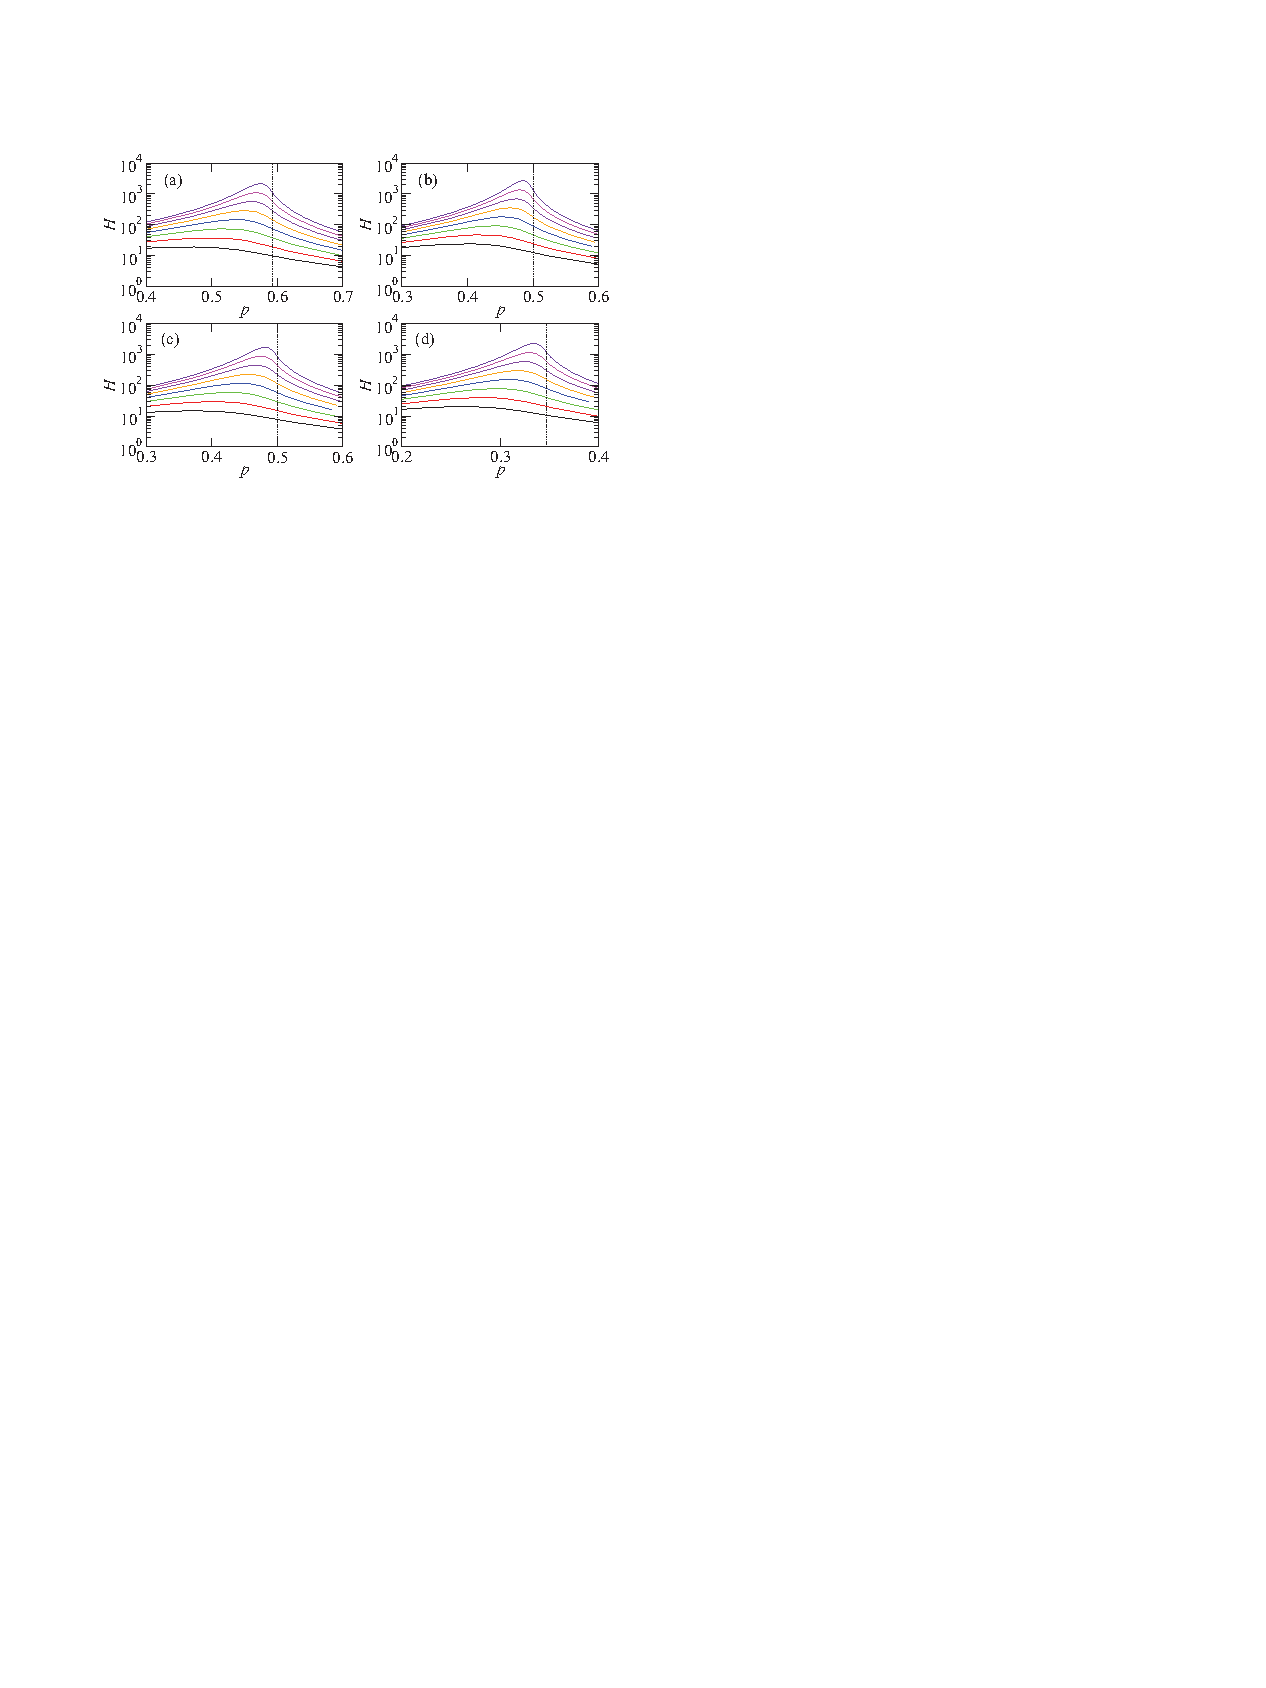
\includegraphics[width=14cm]{img/HetPerc.pdf}
 \caption{Variação da heterogeneidade de tamanhos de domínios em modelos de percolação de sítios em (a) e (c) e de ligações em (b) e (d), na rede quadrada em (a) e (b), e na rede triangular em (c) e (d). A linha pontilhada representa o limiar de percolação. Os tamanhos de rede são $L=2^5, \ldots, 2^{12}$ para a rede quadrada e $L=27 \times 2^0, \ldots, 27 \times 2^7$ para a rede triangular. Quanto maior o valor de $L$, mais alto o valor de $H$~\cite{NohLeePark}.}
\label{fig.HetPerc}
\vspace{8mm}
 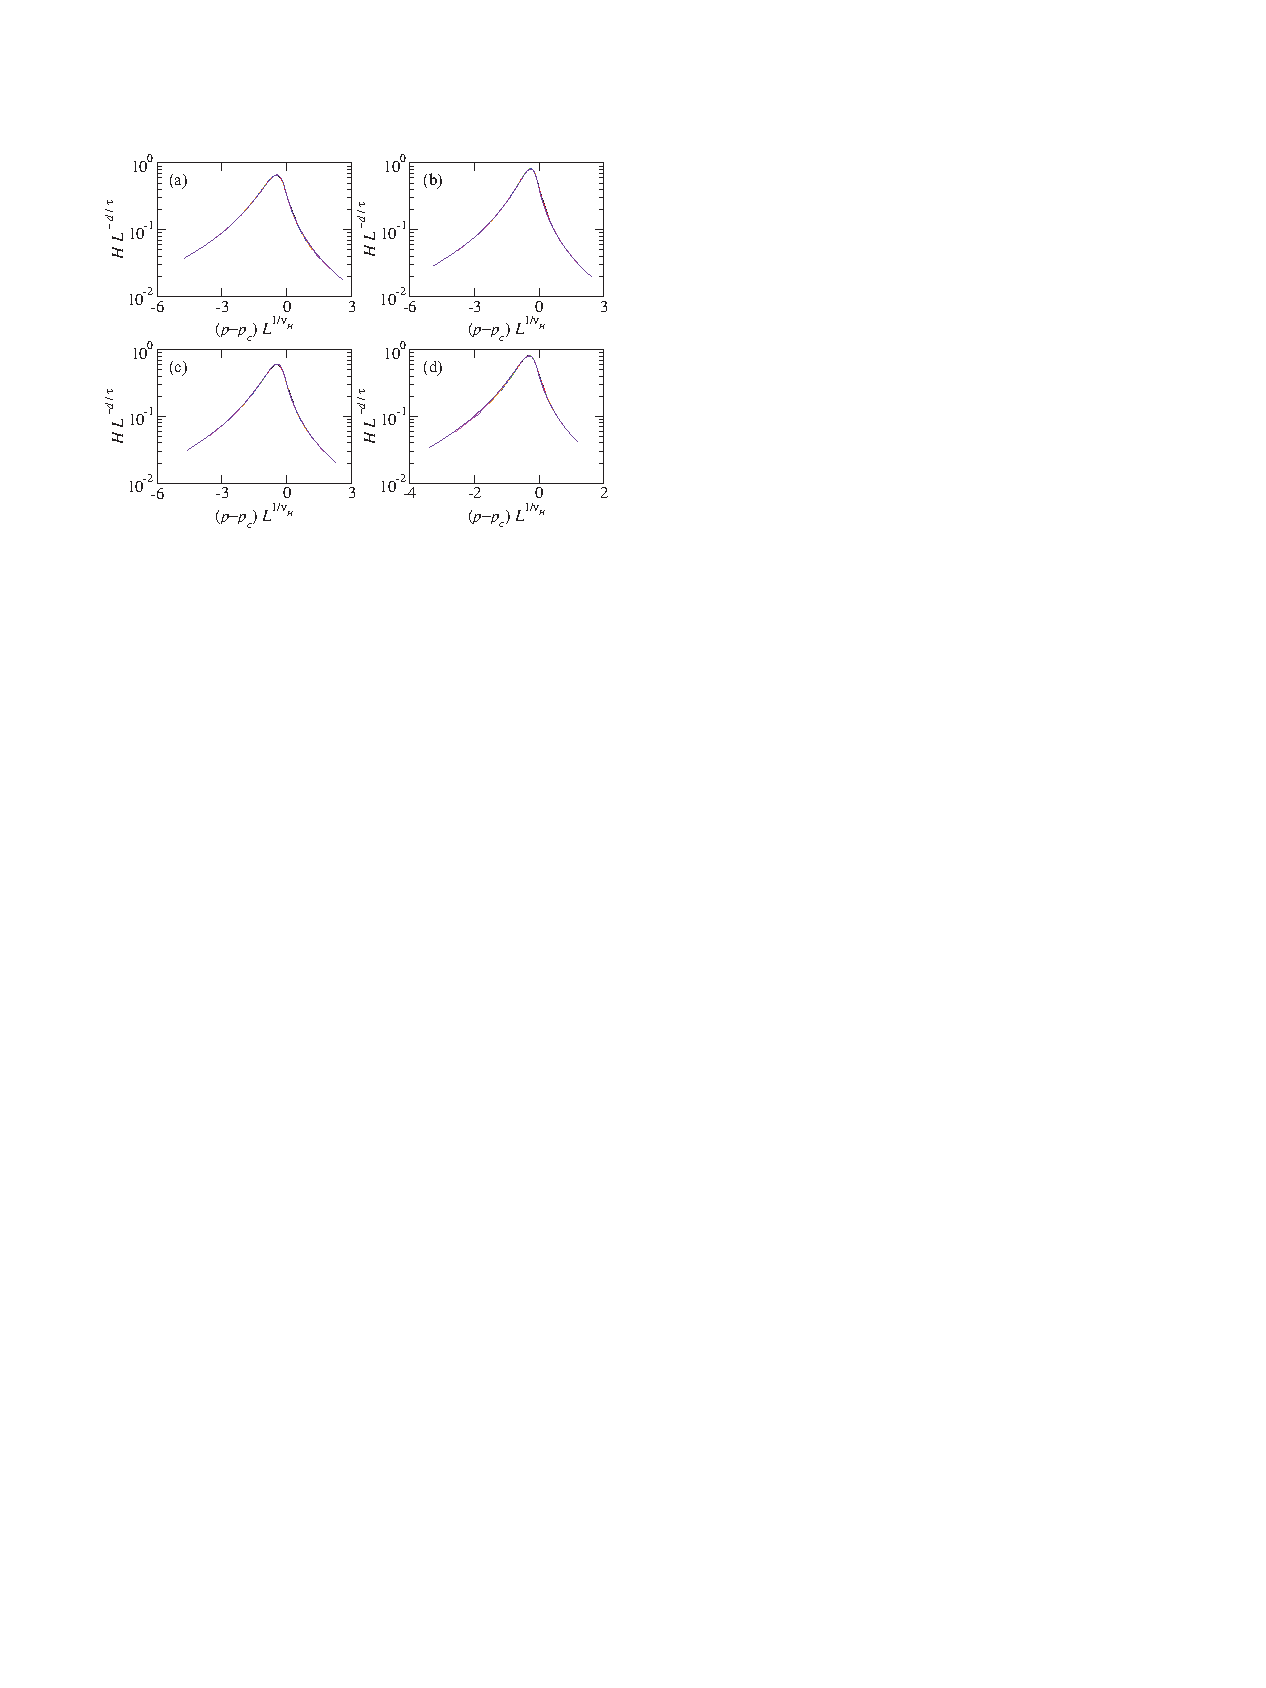
\includegraphics[width=14cm]{img/HetPercCol.pdf}
 \caption{Análise de escala da heterogeneidade de tamanhos de domínios em modelos de percolação de sítios em (a) e (c) e de ligações em (b) e (d), na rede quadrada em (a) e (b), e na rede triangular em (c) e (d). Os dados são os mesmos utilizados na figura \ref{fig.HetPerc}~\cite{NohLeePark}.}
\label{fig.HetPercCol}
\end{figure}


\section{Heterogeneidade no modelo de Ising}

Jo \textit{et al}~\cite{JoYiBaekKim} estudaram a heterogeneidade de tamanhos de domínios geométricos no modelo de Ising em duas dimensões, verificando a validade da forma de escala dada pela Eq.~(\ref{eq.HetPerc}), com a troca do parâmetro $\epsilon$ por $t \equiv (T-T_c)/T_c$, e determinando numericamente o valor do expoente $\nu_H$, através de simulações de Monte Carlo, obtendo um resultado em excelente concordância com o valor $\nu_H = 379/192$, determinado analiticamente com base em expoentes obtidos via teoria de campo conforme (\textit{conformal field theory} - CFT). A figura \ref{fig.IsingH} mostra a variação da heterogeneidade de tamanhos de domínios geométricos no modelo de Ising em duas dimensões, em uma rede quadrada, para estados de equilíbrio, com a variação da temperatura, para vários tamanhos de rede, com dados obtidos através de simulações de Monte Carlo. A figura~\ref{fig.IsingHCol} mostra o colapso dos mesmos dados, de acordo com a forma da Eq.~(\ref{eq.HetPerc}) e do valor obtido para o expoente $\nu_H$.

\begin{figure}
 \centering
 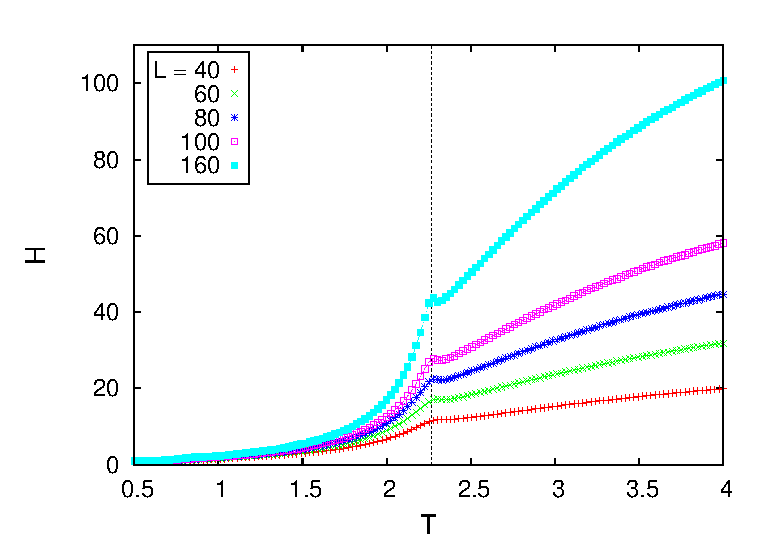
\includegraphics[width=14cm]{fig/hetequi_q2.eps}
 \caption{Heterogeneidade de tamanhos de domínios geométricos no modelo de Ising em duas dimensões, na rede quadrada, em estados de equilíbrio, em função da temperatura, para diversos tamanhos de rede. A linha pontilhada indica a temperatura crítica $T_c$.}
\label{fig.IsingH}
\vspace{8mm}
 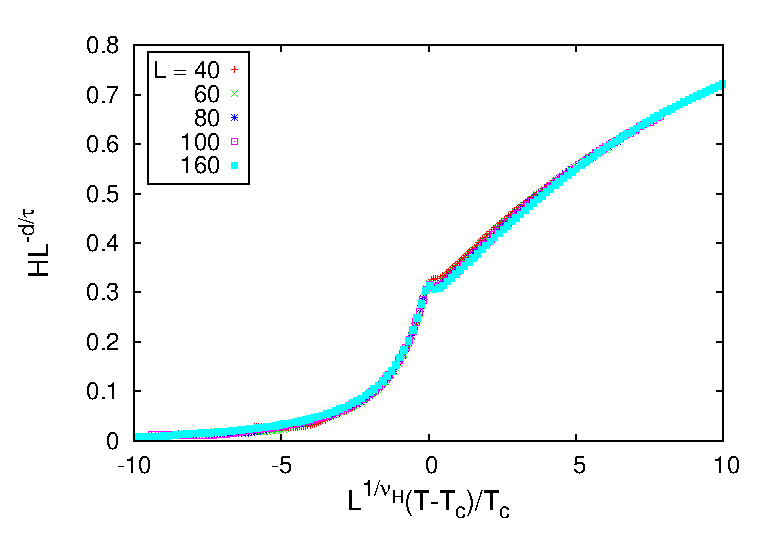
\includegraphics[width=14cm]{fig/hetequi_q2_colXY.eps}
 \caption{Análise de escala da heterogeneidade de tamanhos de domínios geométricos no modelo de Ising em duas dimensões, na rede quadrada, em estados de equilíbrio, em função da temperatura. Os dados são os mesmos utilizados na figura \ref{fig.IsingH}.}
\label{fig.IsingHCol}
\end{figure}


\chapter{Heterogeneidade na dinâmica}
\label{cap.HetDinamica}
 
\section{Introdução}

No capítulo~\ref{cap.Heterogeneidade} foi introduzido o conceito de heterogeneidade de tamanhos de domínios, inicialmente dentro do contexto do modelo de percolação explosiva, onde essa medida, desempenhando o papel de um observável que sinaliza a ocorrência de uma transição de fase, se revelou um importante instrumento na determinação do caráter contínuo da transição observada no modelo. O sucesso do uso da heterogeneidade, nesse contexto, motivou o estudo detalhado de suas propriedades de escala, bem como a sua aplicação nos modelos de percolação de sítios e de ligações, e ainda nos modelos de Ising e Potts. Esses estudos, nos quais a heterogeneidade foi analisada em estados de equilíbrio, tornam natural o questionamento a respeito de sua possível aplicação a sistemas que se encontram fora do equilíbrio, motivando um estudo com a finalidade de tentar caracterizar suas propriedades dinâmicas, e determinar que tipo de informações a mesma poderia fornecer sobre sistemas nessas condições.

Como fatores adicionais que estimulam o estudo da heterogeneidade em sistemas que se encontram fora do equilíbrio, estão questões ainda em aberto, originadas em trabalhos sobre a dinâmica desses sistemas, e a possibilidade que essa medida possa se mostrar útil na elucidação das mesmas. Como um exemplo, temos o comportamento inesperado da distribuição de tamanhos de domínios no modelo de Potts com $q=3$, apresentado no capítulo~\ref{cap.Crescimento}, que evolui após um \textit{quench}, a partir da temperatura crítica, de uma forma compatível com a dinâmica descrita pela Eq.~(\ref{eq.dq2tTc}), embora a mesma, em princípio, seja apenas aplicável ao caso $q=2$.

O estudo das propriedades da heterogeneidade de tamanhos de domínios na dinâmica do modelo de Potts, apresentado neste trabalho, foi baseado em simulações numéricas utilizando o método de Monte Carlo, em uma rede bidimensional quadrada com condições periódicas de contorno, para diversos tamanhos de rede e três diferentes protocolos de \textit{quench}: da temperatura crítica $T_c$ para $T_c/2$, da temperatura infinita para $T_c/2$, e da temperatura infinita para $T_c$, conforme ilustrado na figura~\ref{fig.temperaturas}.

\begin{figure}[h!]
 \setlength\fboxsep{10pt}
 \setlength\fboxrule{0.5pt}
 \centering
 \fbox{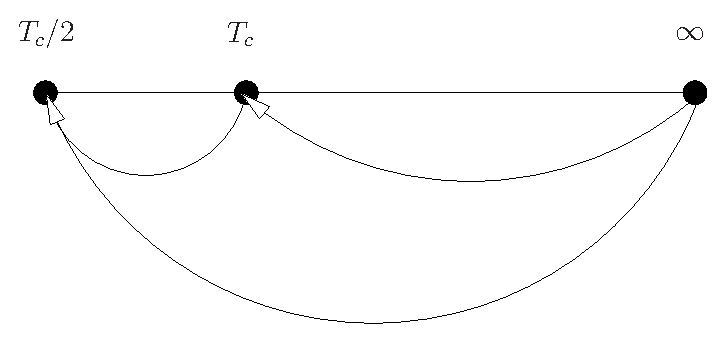
\includegraphics[width=14cm]{img/temperaturas.eps}}
 \caption{Diferentes protocolos de \textit{quench} utilizados nas simulações.}
\label{fig.temperaturas}
\end{figure}


\section{Temperatura inicial crítica e $q=2$}
\label{sec.TcQ2}

Na figura \ref{fig.het_q2_Tc_Tc2} é apresentado o gráfico da heterogeneidade ($H$) de tamanhos de domínios geométricos, para $q=2$, na rede quadrada, durante a evolução do sistema, após um \textit{quench} a partir da temperatura crítica para $T_f=T_c/2$. São apresentadas medidas para tamanhos lineares $L=32, 64, 128, 256, 512$ e $1024$. Os tempos $t$ são medidos a partir do \textit{quench}, em passos de Monte Carlo (MCs), onde cada passo corresponde a $N$ tentativas aleatórias de atualizar o estado dos spins, sendo $N$ o número total de spins na rede.

Na simulação, os spins foram inicialmente escolhidos de forma aleatória, entre os dois valores possíveis, sendo o sistema então submetido a um processo de termalização, que consistiu em permitir a evolução do mesmo, na temperatura crítica, durante um intervalo de tempo suficiente para que pudesse ser considerado em equilíbrio. O sistema foi então submetido ao \textit{quench} para a temperatura $T_f=T_c/2$, e, a partir desse ponto, a simulação da dinâmica foi feita através do algoritmo do \textit{banho térmico}~\cite{Newman}. Após a realização de determinado número de passos de Monte Carlo ($t=2^0..2^{10}$), o conjunto de domínios geométricos presentes no sistema foi determinado, através do algoritmo de Hoshen-Kopelman~\cite{HoshenKopelman}. A partir da configuração de domínios, foi produzida para cada passo uma medida da heterogeneidade de tamanhos de domínios, bem como uma medida da distribuição desses tamanhos. Para cada tempo foi feita uma média sobre até 1000 amostras.

Para simular a dinâmica do sistema durante o processo de termalização, foi empregado o algoritmo de Swendsen-Wang~\cite{SwendsenWang}. Este algoritmo é baseado na construção de aglomerados físicos, conforme descritos por Fortuin e Kasteleyn~\cite{FortuinKasteleyn} e Coniglio e Klein~\cite{ConiglioKlein}, que são então atualizados, sendo o estado de cada spin do aglomerado atualizado para um mesmo valor, entre os dois valores possíveis, escolhido de forma aleatória com igual probabilidade. Cada atualização de todos os aglomerados físicos do sistema é denominada passo de Swendsen-Wang. O número de passos necessários para que o sistema atingisse o equilíbrio na temperatura crítica foi fixado em 500 passos de Swendsen-Wang, em concordância com o protocolo descrito na Ref.~\cite{TeseMP}. A utilização de um algoritmo como o de Swendsen-Wang se justifica pelo fato de o mesmo ser consideravelmente mais eficiente que algoritmos do tipo \textit{single-flip}, como o de Metropolis e do banho térmico, nas proximidades do ponto crítico, por serem estes muito suscetíveis ao fenômeno conhecido como desaceleração crítica, ou ralentamento crítico, que torna a dinâmica do sistema extremamente lenta nessa região. No entanto, embora o algoritmo de Swendsen-Wang seja útil para levar o sistema rapidamente a um estado de equilíbrio, o que é desejável na etapa de termalização, o mesmo tem uma dinâmica não-local, o que impede a sua utilização na etapa após o \textit{quench} para $T_f=T_c/2$, onde se realizam medidas enquanto o sistema evolui fora do equilíbrio, o que explica a utilização de dois diferentes algoritmos de Monte Carlo, nas diferentes etapas da simulação. 

Observando-se o gráfico apresentado na figura \ref{fig.het_q2_Tc_Tc2}, é possível perceber que as curvas apresentam dois comportamentos distintos, visíveis para grandes tamanhos de rede. Para tempos pequenos, $H$ se mantém aproximadamente constante, enquanto que, a partir de um certo ponto, parece decair como uma lei de potência. Com o objetivo de tentar obter informações sobre o comportamento de $H$, e determinar a sua forma de escala, foi construído o gráfico apresentado na figura~\ref{fig.het_q2_Tc_Tc2_colXY}. O eixo vertical foi reescalado como $H \rightarrow HL^{-d/\tau}$. Essa forma era esperada, pelo fato de a heterogeneidade no tempo $t=0$ ser equivalente à heterogeneidade do sistema em equilíbrio, $H(t=0)=H_{\scriptstyle\rm eq}(T_c)$, cuja forma de escala foi determinada para o modelo de Ising, utilizando-se escalamento de tamanhos finitos, conforme apresentado no capítulo~\ref{cap.Heterogeneidade}, e ilustrado pelo colapso obtido na figura~\ref{fig.IsingHCol}. Nessa expressão, $d$ é a dimensão do sistema e $\tau$ é um expoente que caracteriza o tamanho dos domínios. Utilizou-se $\tau = 187/91$, que é o valor exato para domínios geométricos no modelo de Ising, para a temperatura crítica~\cite{PRLJeferson,PREJeferson}. O eixo horizontal foi reescalado como $t \rightarrow t/L$. Conforme pode ser observado na figura~\ref{fig.het_q2_Tc_Tc2_colXY}, as curvas de $H$ parecem convergir assintoticamente para uma mesma reta, com o aumento do tamanho do sistema, indicando um comportamento do tipo lei de potência no limite termodinâmico. A justificativa para o desvio da lei de potência parece residir no fato que sistemas menores chegam antes a um estado magnetizado, com domínios associados às flutuações térmicas, o que faz com que $H$ atinja um valor estacionário. No limite termodinâmico, o tempo para cair em um estado magnetizado diverge, e se esperaria a convergência de $H$ para a lei de potência. A linha reta pontilhada, apresentada no gráfico, tem uma declividade aproximadamente igual a $-0.82$, determinada através de ajuste aos dados da curva de $H$ para $L=1024$. No entanto, serão necessários resultados obtidos com sistemas maiores, para que se possa obter um valor próximo ao esperado para o expoente no limite termodinâmico.

\begin{figure}[p]
 \centering
 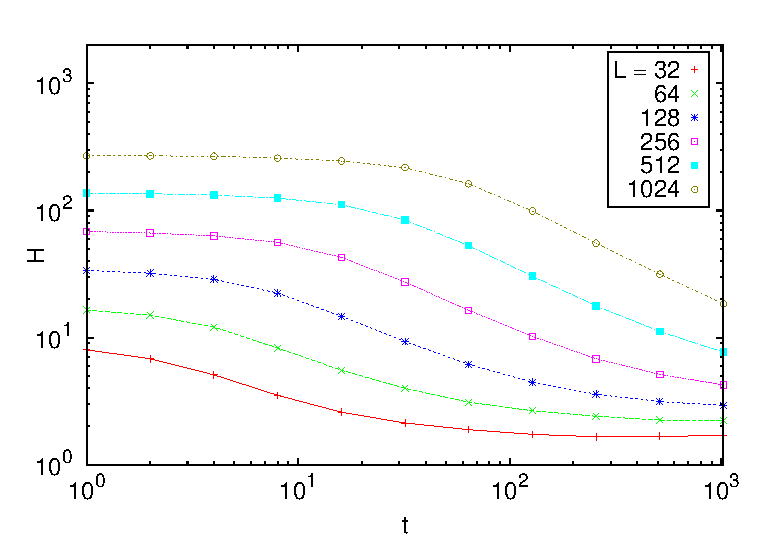
\includegraphics[width=14cm]{fig/het_q2_Tc_Tc2.eps}
 \caption{Variação da heterogeneidade de tamanhos de domínios geométricos para o modelo de Ising na rede quadrada, após um \textit{quench} de $T_0=T_c$ para $T_f=T_c/2$, para diferentes valores de $L$.}
\label{fig.het_q2_Tc_Tc2}
\vspace{8mm}
 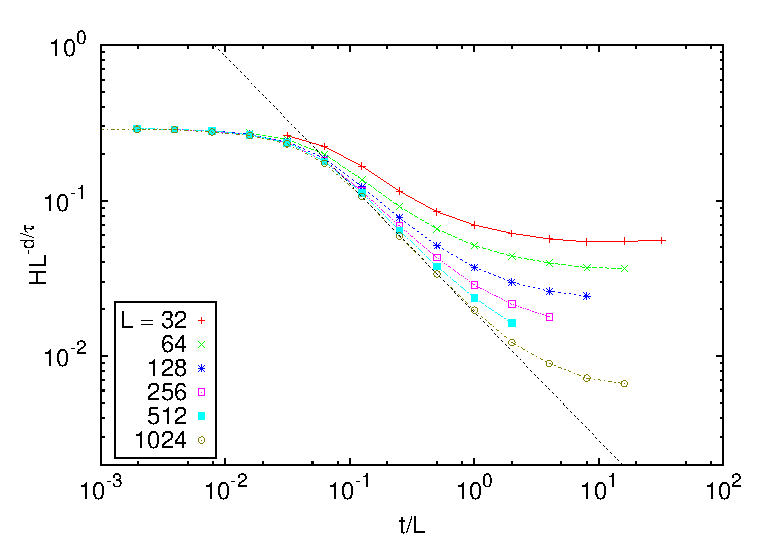
\includegraphics[width=14cm]{fig/het_q2_Tc_Tc2_colXY.eps}
 \caption{Análise de escala da heterogeneidade de tamanhos de domínios geométricos para o modelo de Ising na rede quadrada, após um \textit{quench} de $T_0=T_c$ para $T_f=T_c/2$. Os dados são os mesmos utilizados na figura~\ref{fig.het_q2_Tc_Tc2}. A linha reta pontilhada tem declividade $-0.82$.}
\label{fig.het_q2_Tc_Tc2_colXY}
\end{figure}


\section{Temperatura inicial infinita e $q=2$}
\label{sec.TinfQ2}

Na figura \ref{fig.het_q2_Tinf_Tc2} é apresentado o gráfico da heterogeneidade de tamanhos de domínios geométricos, para $q=2$, após um \textit{quench} a partir da temperatura infinita para $T_f=T_c/2$. Como no caso anterior, são apresentadas medidas para tamanhos lineares $L=32, 64, 128, 256, 512$ e $1024$. A temperatura inicial infinita equivale a um estado onde os spins estão totalmente descorrelacionados, sendo cada um dos mesmos escolhido de forma aleatória entre os dois valores possíveis. A simulação da dinâmica, após o \textit{quench}, foi feita através do algoritmo do banho térmico, sendo as medidas realizadas exatamente como descrito para o caso com temperatura inicial crítica.

Assim como apresentado na seção~\ref{sec.TcQ2}, foi feita uma tentativa de se determinar a forma de escala de $H$ neste caso, sendo o eixo vertical reescalado como $H \rightarrow HL^{-d/\tau}$ e o horizontal como $t \rightarrow t/L$. Utilizou-se $\tau = 379/187$, que é o valor exato para domínios geométricos no modelo de Ising, para a temperatura infinita~\cite{PRLJeferson,PREJeferson}. O resultado pode ser observado na figura~\ref{fig.het_q2_Tinf_Tc2_colXY}. Mais uma vez, parece que temos um colapso progressivo das curvas, com uma convergência assintótica para uma lei de potência, com o aumento do tamanho do sistema. Percebe-se ainda, no comportamento de $H$, um pequeno decaimento inicial, atribuído ao fato de que neste caso, em um ou dois passos de Monte Carlo, o sistema atinge o estado crítico percolativo~\cite{PRLJeferson}, o que leva ao aparecimento de um domínio percolante, que ocupa uma fração considerável da rede, diminuindo a quantidade e diversidade dos domínios (apesar da distribuição ficar mais larga). A linha reta pontilhada, apresentada no gráfico, tem uma declividade aproximadamente igual a $-0.85$, determinada através de ajuste aos dados da curva de $H$ para $L=1024$.

\begin{figure}[p]
 \centering
 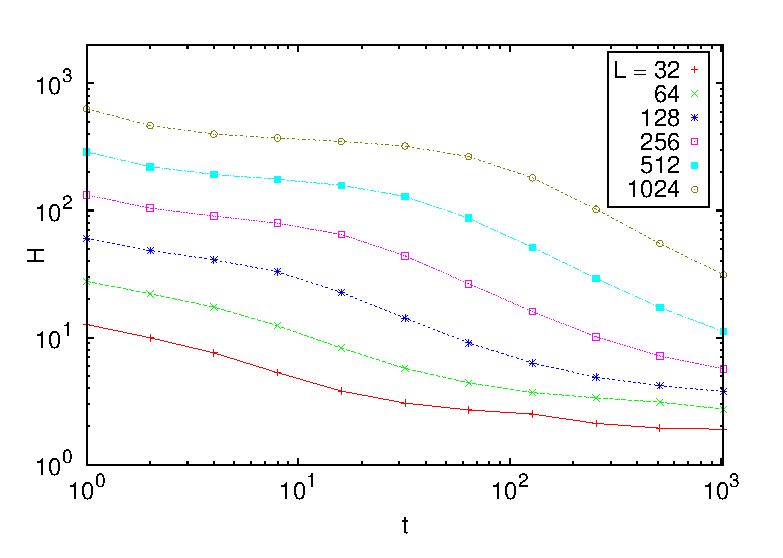
\includegraphics[width=14cm]{fig/het_q2_Tinf_Tc2.eps}
 \caption{Variação da heterogeneidade de tamanhos de domínios geométricos para o modelo de Ising na rede quadrada, após um \textit{quench} de $T_0\rightarrow \infty$ para $T_f=T_c/2$, para diferentes valores de $L$.}
\label{fig.het_q2_Tinf_Tc2}
\vspace{8mm}
 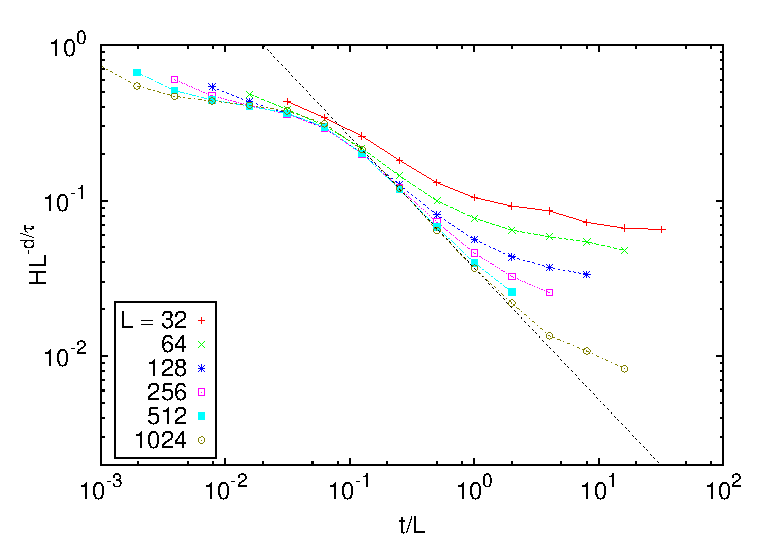
\includegraphics[width=14cm]{fig/het_q2_Tinf_Tc2_colXY.eps}
 \caption{Análise de escala da heterogeneidade de tamanhos de domínios geométricos para o modelo de Ising na rede quadrada, após um \textit{quench} de $T_0\rightarrow \infty$ para $T_f=T_c/2$. Os dados são os mesmos utilizados na figura~\ref{fig.het_q2_Tinf_Tc2}. A linha reta pontilhada tem declividade $-0.85$.}
\label{fig.het_q2_Tinf_Tc2_colXY}
\end{figure}


\section{Temperatura inicial crítica e $q=3$}
\label{sec.TcQ3}

Na figura \ref{fig.het_q3_Tc_Tc2} é apresentado o gráfico da heterogeneidade de tamanhos de domínios geométricos, para $q=3$, na rede quadrada, durante a evolução do sistema, após um \textit{quench} a partir da temperatura crítica para $T_f=T_c/2$. São apresentadas medidas para tamanhos lineares $L=32, 64, 128, 256, 512$ e $1024$. O procedimento adotado na simulação foi análogo ao apresentado na seção \ref{sec.TcQ2}.

Mais uma vez, foi feita uma tentativa de se determinar a forma de escala de $H$, sendo o eixo vertical reescalado como $H \rightarrow HL^{-d/\tau}$ e o horizontal como $t \rightarrow t/L$. Utilizou-se $\tau = 187/91$, que é o valor exato para domínios geométricos no modelo de Ising, para a temperatura crítica~\cite{PRLJeferson,PREJeferson}. Para domínios geométricos no modelo de Potts, com $q=3$, o valor de $\tau$ não é conhecido exatamente, mas é bastante próximo ao encontrado para o modelo de Ising~\cite{LoureiroPRE}. O resultado pode ser observado na figura~\ref{fig.het_q3_Tc_Tc2_colXY}. Novamente, as curvas de $H$ parecem convergir assintoticamente para uma mesma reta, com o aumento do tamanho do sistema, indicando um comportamento do tipo lei de potência no limite termodinâmico. A linha reta pontilhada, apresentada no gráfico, tem uma declividade aproximadamente igual a $-0.82$, determinada através de ajuste aos dados da curva de $H$ para $L=1024$.

\begin{figure}[p]
 \centering
 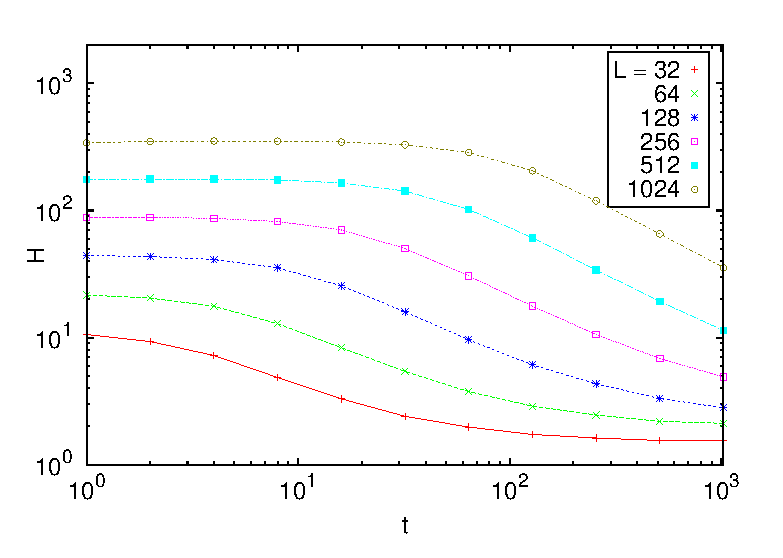
\includegraphics[width=14cm]{fig/het_q3_Tc_Tc2.eps}
 \caption{Variação da heterogeneidade de tamanhos de domínios geométricos para o modelo de Potts na rede quadrada, com $q=3$, após um \textit{quench} de $T_0=T_c$ para $T_f=T_c/2$, para diferentes valores de $L$.}
\label{fig.het_q3_Tc_Tc2}
\vspace{8mm}
 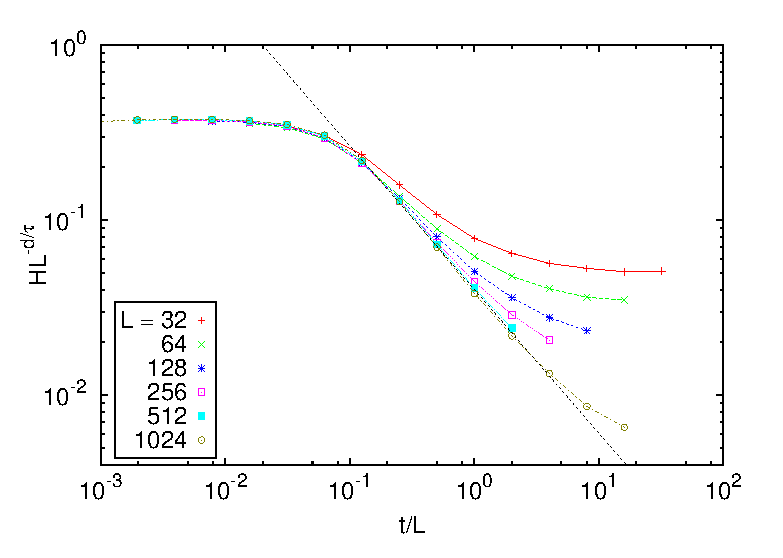
\includegraphics[width=14cm]{fig/het_q3_Tc_Tc2_colXY.eps}
 \caption{Análise de escala da heterogeneidade de tamanhos de domínios geométricos para o modelo de Potts na rede quadrada, com $q=3$, após um \textit{quench} de $T_0=T_c$ para $T_f=T_c/2$. Os dados são os mesmos utilizados na figura~\ref{fig.het_q3_Tc_Tc2}. A linha reta pontilhada tem declividade $-0.82$.}
\label{fig.het_q3_Tc_Tc2_colXY}
\end{figure}


\section{Temperatura inicial infinita e $q=3$}
\label{sec.TinfQ3}

Na figura \ref{fig.het_q3_Tinf_Tc2} é apresentado o gráfico da heterogeneidade de tamanhos de domínios geométricos, para $q=3$, na rede quadrada, durante a evolução do sistema, após um \textit{quench} a partir da temperatura infinita para $T_f=T_c/2$. São apresentadas medidas para tamanhos lineares $L=32, 64, 128, 256, 512$ e $1024$. O procedimento adotado na simulação foi análogo ao apresentado na seção~\ref{sec.TinfQ2}. Em relação aos casos anteriores, percebe-se uma diferença qualitativa: enquanto nos demais casos as curvas parecem ser estritamente decrescentes, neste as curvas claramente possuem um ponto máximo. Com o objetivo de se obter mais informações sobre esse máximo, é apresentado na figura~\ref{fig.hetevlin_q3_Tinf_Tc2} um gráfico linear, no qual $H$ foi medido para todos os passos de Monte Carlo, o que facilita a determinação das posições onde ocorrem os máximos nas curvas (indicados por segmentos de reta verticais). Na figura~\ref{fig.areasev_q3_L512_Tinf_Tc2}, observamos ainda o gráfico das distribuições para este caso, com $L=512$, utilizando os mesmos dados usados na construção da figura~\ref{fig.hetevlin_q3_Tinf_Tc2}, com a curva para o tempo em que ocorre o máximo valor de $H$ em destaque. Aparentemente, não é possível perceber através da curva da distribuição qualquer particularidade que indique um correspondente máximo na heterogeneidade.

\begin{figure}[p]
 \centering
 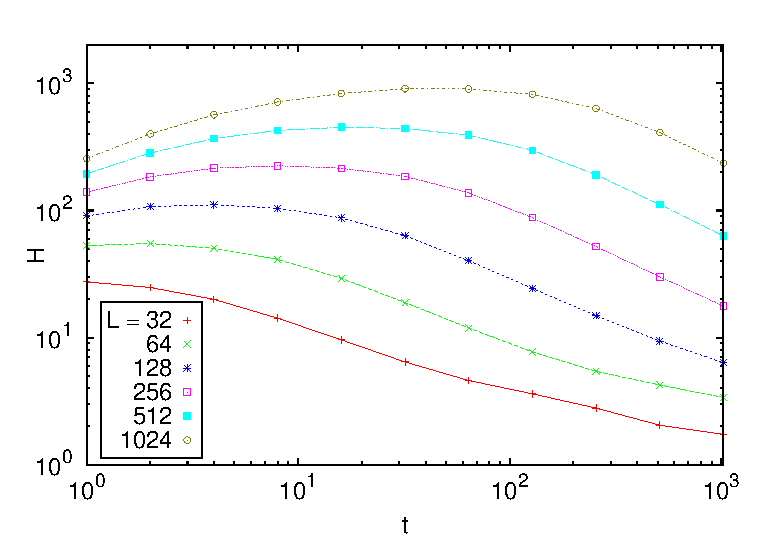
\includegraphics[width=14cm]{fig/het_q3_Tinf_Tc2.eps}
 \caption{Variação da heterogeneidade de tamanhos de domínios geométricos para o modelo de Potts na rede quadrada, com $q=3$, após um \textit{quench} de $T_0\rightarrow \infty$ para $T_f=T_c/2$, para diferentes valores de $L$.}
\label{fig.het_q3_Tinf_Tc2}
\vspace{8mm}
 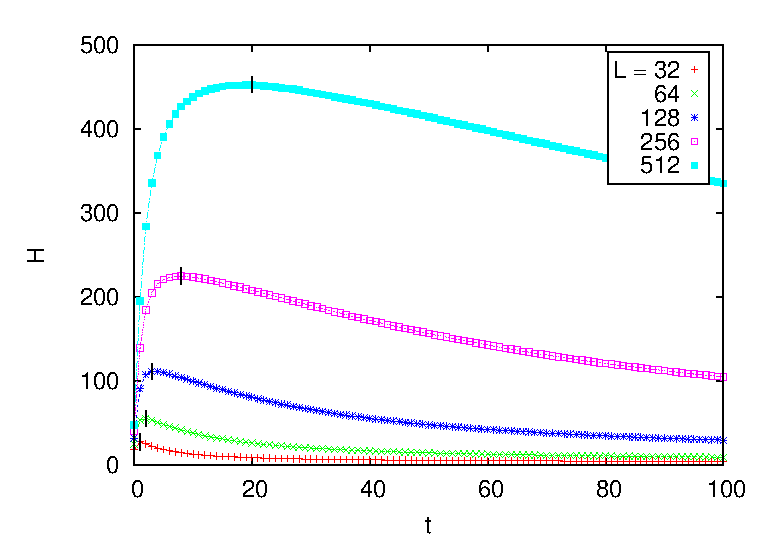
\includegraphics[width=14cm]{fig/hetevlin_q3_Tinf_Tc2.eps}
 \caption{Gráfico linear da heterogeneidade de tamanhos de domínios geométricos para o modelo de Potts na rede quadrada, com $q=3$, após um \textit{quench} de $T_0\rightarrow \infty$ para $T_f=T_c/2$, para diferentes valores de $L$, com a posição aproximada dos máximos indicada por segmentos de reta verticais.}
\label{fig.hetevlin_q3_Tinf_Tc2}
\end{figure}

Como nos casos anteriores, foi feita uma tentativa de se determinar a forma de escala de $H$, sendo o eixo vertical reescalado como $H \rightarrow HL^{-d/\tau}$ e o horizontal como $t \rightarrow t/L$. Utilizou-se $\tau = 379/187$, que é o valor exato para domínios geométricos no modelo de Ising, para a temperatura infinita~\cite{PRLJeferson,PREJeferson}, como uma aproximação para o caso com $q=3$, justificada pela proximidade dos valores~\cite{LoureiroPRE}. O resultado pode ser observado na figura~\ref{fig.het_q3_Tinf_Tc2_colXY}. Mais uma vez, parece que temos um colapso progressivo das curvas, com uma convergência assintótica para uma lei de potência, com o aumento do tamanho do sistema. A linha reta pontilhada, apresentada no gráfico, tem uma declividade aproximadamente igual a $-0.87$, determinada através de ajuste aos dados da curva de $H$ para $L=1024$.

\begin{figure}[p]
 \centering
 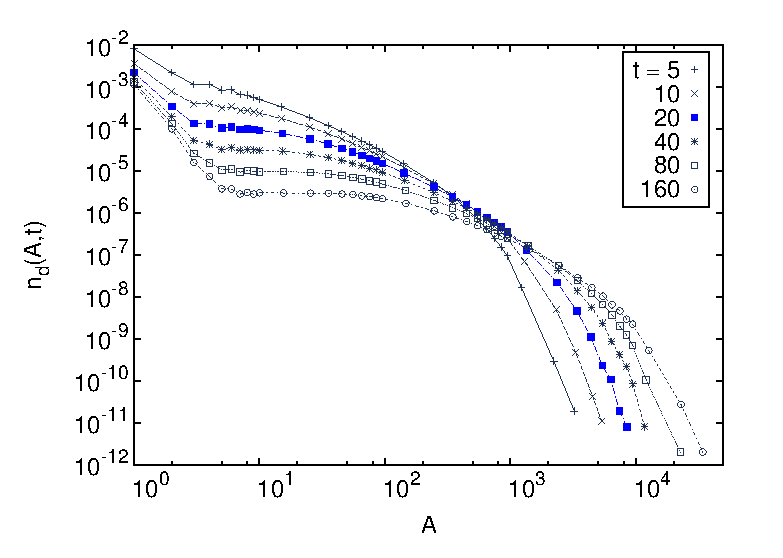
\includegraphics[width=14cm]{fig/areasev_q3_L512_Tinf_Tc2.eps}
 \caption{Distribuições de tamanhos de domínios geométricos para o modelo de Potts na rede quadrada, com $q=3$ e $L=512$, após um \textit{quench} de $T_0\rightarrow \infty$ para $T_f=T_c/2$, para diferentes tempos, utilizando os mesmos dados usados na construção da figura~\ref{fig.hetevlin_q3_Tinf_Tc2}, com a curva para o tempo $t=20$, em que ocorre o máximo valor de $H$, em destaque.}
\label{fig.areasev_q3_L512_Tinf_Tc2}
\vspace{8mm}
 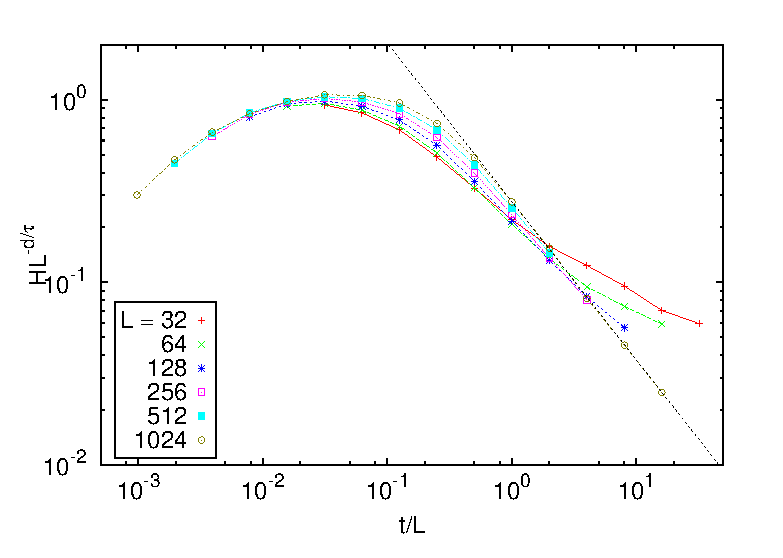
\includegraphics[width=14cm]{fig/het_q3_Tinf_Tc2_colXY.eps}
 \caption{Análise de escala da heterogeneidade de tamanhos de domínios geométricos para o modelo de Potts na rede quadrada, com $q=3$, após um \textit{quench} de $T_0\rightarrow \infty$ para $T_f=T_c/2$. Os dados são os mesmos utilizados na figura~\ref{fig.het_q3_Tinf_Tc2}. A linha reta pontilhada tem declividade $-0.87$.}
\label{fig.het_q3_Tinf_Tc2_colXY}
\end{figure}


\section{Temperatura inicial infinita e temperatura final crítica}

Com a finalidade de verificar se o comportamento caracterizado pela presença de um máximo na variação da heterogeneidade ocorre também em outros protocolos de \textit{quench} que partem da temperatura infinita, foram realizadas simulações onde o \textit{quench} foi feito de $T_0\rightarrow \infty$ para $T_f=T_c$, para $q=2$ e $q=3$. A escolha desse particular protocolo foi sugerida pelo recente trabalho de Blanchard \textit{et al}~\cite{BlanchardCugliandoloPicco}, no qual o mesmo foi utilizado no estudo de propriedades dinâmicas do modelo de Ising, embora com diferentes tipos de domínios ou geometrias de rede. O resultado obtido pode ser observado na figura~\ref{fig.het_L1024_Tc_lines}, onde se pode perceber a presença de um máximo na curva de $H$, para $q=3$. As linhas retas pontilhadas, apresentadas no gráfico, são paralelas, com uma declividade aproximadamente igual a $-0.21$, determinada através de ajuste aos dados obtidos para $q=3$. Entretanto, para que seja possível verificar a forma de convergência assintótica das curvas, e ainda, no caso de uma lei de potência, determinar o valor do expoente, serão necessárias simulações adicionais, para diferentes tamanhos de rede, bem como uma análise do colapso dos dados obtidos.

\begin{figure}[h!]
 \centering
 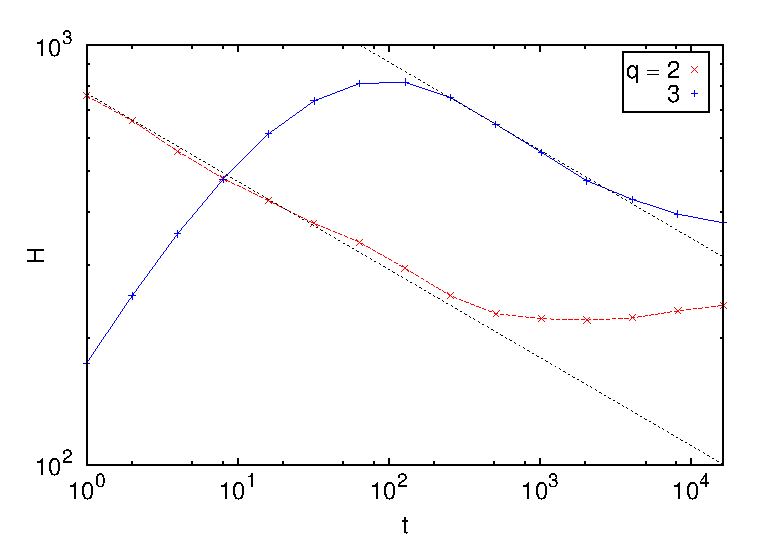
\includegraphics[width=14cm]{fig/het_L1024_Tc_lines.eps}
 \caption{Variação da heterogeneidade de tamanhos de domínios geométricos para o modelo de Potts na rede quadrada, para $q=2$ e $q=3$, após um \textit{quench} de $T_0\rightarrow \infty$ para $T_f=T_c$, para $L=1024$. As linhas retas pontilhadas são paralelas, com declividade $-0.21$.}
\label{fig.het_L1024_Tc_lines}
\end{figure}


\section{Comparações entre diferentes protocolos de \textit{quench}}

As diferenças no comportamento dinâmico da heterogeneidade, para os diferentes protocolos de \textit{quench} estudados, tornam-se mais perceptíveis quando as curvas obtidas em cada caso, para um mesmo tamanho de rede, são apresentadas no mesmo gráfico, como pode ser observado na figura~\ref{fig.het_L1024_Tc2_lines}, gerada para $L=1024$. Percebe-se claramente a diferença qualitativa, já mencionada, da existência de um máximo na curva, no caso em que $q=3$ e $T_0\rightarrow \infty$, contrastando com o comportamento estritamente decrescente nos demais casos. Apesar dessa diferença, pode-se observar que todas as curvas parecem convergir, para tempos grandes, para retas com aproximadamente a mesma declividade, sugerindo um comportamento do tipo lei de potência, com o mesmo expoente para todos os casos. As linhas retas pontilhadas, apresentadas no gráfico, são todas paralelas, com uma declividade aproximadamente igual a $-0.86$, determinada através de ajuste aos dados obtidos para $q=3$ e $T_0\rightarrow \infty$. Essas retas, no entanto, são indicativas do comportamento para esse particular tamanho de rede, não necessariamente refletindo o que se obteria no limite termodinâmico. Para se reduzir o erro na determinação do valor do expoente, serão necessárias simulações adicionais, para permitir uma análise de escala com tamanhos de rede maiores.

Nota-se ainda que as curvas para os casos onde $q=2$, $T_0\rightarrow \infty$, e $q=3$, $T_0=T_c$, estão praticamente colapsadas, enquanto que no caso onde $q=2$ e $T_0=T_c$, embora a curva tenha uma forma semelhante, está deslocada em relação às demais. Pode-se obter um colapso aproximado desta última curva sobre as primeiras, multiplicando-se o valor de $H$ por um fator aproximadamente igual a $2$. Atribuímos esse comportamento ao fator $2$ que aparece na expressão da distribuição para o caso $q=2$, $T_0\rightarrow \infty$, mas não no caso $q=2$, $T_0=T_c$, conforme pode ser observado nas Eq.~(\ref{eq.dq2tTinf}) e (\ref{eq.dq2tTc}), e também a um fator 2 que aparece na distribuição determinada heuristicamente por Loureiro \textit{et al}, que se ajusta aos dados obtidos para $q=3$~\cite{LoureiroPRE}. Desta maneira, ao aumentar a probabilidade de uma determinada área na distribuição, aumenta sua probabilidade de aparecer em uma amostra e contribuir para o valor de $H$.

O caso onde $q=3$ e $T_0\rightarrow \infty$, dentre os aqui estudados, é o único a não apresentar uma grande cauda na distribuição, conforme pode ser observado na figura~\ref{fig.AreasCol}. Esperaríamos, em princípio, que o mesmo apresentasse valores de $H$ menores que nos demais casos. Entretanto, se verifica que ocorre o oposto. Como justificativa para esse comportamento, parece estar o fato que neste caso em geral não aparecem domínios percolantes durante o intervalo de tempo considerado, por estar a probabilidade associada a cada variedade de spin, na distribuição aleatória inicial ($1/3$), distante do valor da densidade crítica do modelo de percolação aleatória. Assim, para cada amostra do sistema, neste caso, podem aparecer um grande número de domínios, com uma grande variedade de tamanhos. Já nos demais casos estudados, há uma grande probabilidade de existirem domínios percolantes, seja pelo fato de a configuração inicial do sistema não ter temperatura infinita, estando os spins correlacionados, ou, para o caso onde $q=2$ e $T_0\rightarrow \infty$, pela proximidade da probabilidade associada a cada variedade de spin na distribuição aleatória inicial ($1/2$) com a densidade crítica do modelo de percolação aleatória $\rho_c \sim 0.59$~\cite{PRLJeferson}. Assim, para configurações com um ou mais domínios percolantes ocupando a maior parte do sistema, resta uma pequena área a ser ocupada por domínios menores, levando a uma variedade de tamanhos de domínios consideravelmente menor.

\begin{figure}[h!]
 \centering
 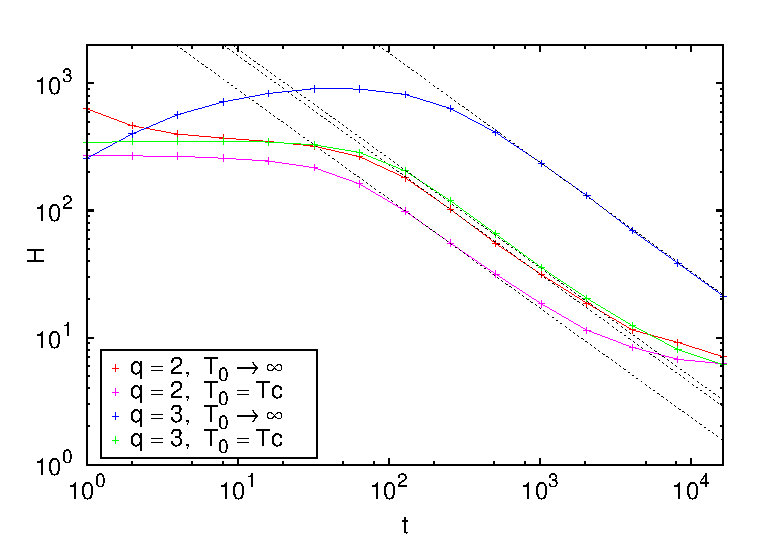
\includegraphics[width=14cm]{fig/het_L1024_Tc2_lines.eps}
 \caption{Variação da heterogeneidade de tamanhos de domínios geométricos para o modelo de Potts na rede quadrada, para diferentes valores de $q$ e temperaturas iniciais, para $L=1024$ e $T_f=T_c/2$. As linhas retas pontilhadas são todas paralelas, com declividade $-0.86$.}
\label{fig.het_L1024_Tc2_lines}
\end{figure}


\chapter{Conclusões}
\label{Conclusoes}

Neste trabalho, estudamos o comportamento da heterogeneidade de tamanhos de domínios ($H$) nos modelos de Ising e Potts, em situações fora do equilíbrio, tentando caracterizar suas propriedades dinâmicas e determinar que tipo de informações a mesma poderia fornecer sobre sistemas nessas condições, motivados por questões em aberto sobre a dinâmica de crescimento de domínios no modelo de Potts, e dando continuidade ao trabalho iniciado por Loureiro \textit{et al}~\cite{LoureiroPRE}. Medimos $H$ durante a evolução do sistema, para diversos tamanhos de rede, após este ser submetido a um \textit{quench}, de acordo com três diferentes protocolos: da temperatura crítica $T_c$ para $T_c/2$, da temperatura infinita para $T_c/2$, e da temperatura infinita para $T_c$. Para cada caso estudado, fizemos uma análise de escala, baseada no conhecimento prévio do comportamento de $H$ para sistemas em equilíbrio, e tentamos interpretar os resultados obtidos, à luz de resultados prévios de estudos sobre crescimento de domínios.

Verificamos que $H$ exibe dois comportamentos distintos, visíveis para grandes tamanhos de rede: para tempos pequenos, $H$ se mantém aproximadamente constante, enquanto que, para tempos maiores, decai como uma lei de potência. Justificamos o desvio em relação ao comportamento do tipo lei de potência, para sistemas menores, pelo fato de que esses sistemas tendem a cair rapidamente em um estado magnetizado, com domínios associados às flutuações térmicas, fazendo com que $H$ atinja um valor estacionário. Tentamos estimar os expoentes associados ao comportamento de lei de potência, para cada caso estudado. Para os casos onde o \textit{quench} foi feito para uma temperatura subcrítica, obtivemos um expoente com valor aproximadamente igual a 0.85, enquanto que nos casos onde o \textit{quench} foi feito para a temperatura crítica, este valor situou-se em torno de 0.2. Entretanto, esses valores, determinados através do ajuste aos dados obtidos para os maiores tamanhos de rede que utilizamos ($L=1024$), devem ser considerados como resultados preliminares, e não como uma estimativa aceitável para os valores esperados no limite termodinâmico. Para que se obtenha resultados mais confiáveis para os expoentes, serão necessárias novas simulações, com redes maiores, bem como tempos mais longos, para permitir uma análise mais precisa. Sobre o valor do expoente para os casos subcríticos, é possível que o mesmo venha a se aproximar de 1, no limite de grandes tamanhos de rede, o que poderia talvez ser explicado com base no comportamento do número esperado de domínios: $\langle N_c \rangle \sim 1/t$, e considerando a hipótese de $H$ depender fortemente desse número. Já para o valor do expoente para os casos em que o \textit{quench} foi feito para a temperatura crítica, não temos ainda nenhuma hipótese, e imaginamos que o mesmo possa ser indicativo de um comportamento não-trivial, relacionado a particularidades da dinâmica crítica.

Comparamos o comportamento de $H$ para os diversos casos estudados, encontrando algumas características significativas. Uma delas foi a presença de um máximo na variação de $H$, para os casos em que o \textit{quench} foi feito a partir da temperatura infinita, para $q=3$, o que contrasta com o comportamento estritamente decrescente, observado nos demais casos. Com base no colapso dos dados, obtido na análise de escala, parece existir uma dependência linear entre o tamanho $L$ da rede e o tempo em que ocorre o máximo. Entretanto, a questão mais fundamental, acerca da origem desse máximo, permanece em aberto. Outra característica observada, é a semelhança da curva de $H$ para $q=3$, no \textit{quench} de $T_0 = T_c$ para $T_f=T_c/2$, com as curvas obtidas para $q=2$, nos casos onde o \textit{quench} foi feito para $T_f=T_c/2$, o que remete ao comportamento análogo, e ainda não elucidado, observado nas distribuições. Sobre esses casos, verificamos ainda que a curva obtida para $q=2$ e $T_0=T_c$ está deslocada em relação às demais, fato que atribuímos à presença ou ausência de um fator $2$ nas correspondentes distribuições, novamente sugerindo uma forte relação entre $H$ e a distribuição.

Como perspectivas para a continuação deste trabalho, temos a confirmação da forma de escala de $H$, e a determinação mais precisa dos valores dos expoentes, através de simulações com redes maiores e tempos mais longos. Seria importante ainda tentar obter uma explicação satisfatória para o comportamento de $H$, em particular para a região em que a curva se mantém aproximadamente constante, ou apresenta um máximo, antes de entrar no regime de lei de potência, e talvez se chegar a expressões exatas que descrevam o comportamento de $H$ e sua relação com as distribuições. Outras possíveis extensões a este trabalho, são o estudo do comportamento de $H$ para o caso de \textit{hulls} ou domínios físicos, ou para valores de $q$ maiores que $3$, bem como para outras dimensões e geometrias de rede.



%\appendix

%bibliografia
\fancyhead{}
\fancyhead[LE,RO]{\scriptsize \slshape \leftmark}
\fancyhead[LO,RE]{\thepage}

\bibliography{Biblio}   
\addcontentsline{toc}{chapter}{Referências Bibliográficas}

\end{document}

